\documentclass[a4paper, 12pt, oneside]{book}
% Dimensiones y márgenes----------------------------------------------
\usepackage[%
    left=1.2in,%
    right=1.2in,%
    top=1.2in,%
    bottom=1.5in,%
    paperheight=11in,%
    paperwidth=8.5in%
]{geometry}
\parindent=0mm
% Otros paquetes -----------------------------------------------------
\usepackage[utf8]{inputenc}
\usepackage{lmodern}
\usepackage{layout}
\usepackage{emptypage}
\usepackage{fancyhdr}

\usepackage{cite}
\usepackage{caption}
\usepackage{mathtools}
\usepackage{hyperref}
\usepackage[all]{xy}
\usepackage{listings}
\usepackage[spanish]{babel}
\usepackage{url}
\usepackage{float}
\usepackage{eurosym}
\usepackage{multirow}
\usepackage{rotating} 
\usepackage{color}
\usepackage{titlesec}
\usepackage{colortbl}
\usepackage[table]{xcolor}
\usepackage[spanish]{babel}
\usepackage{enumerate}
\usepackage{subfig}
\usepackage{afterpage}
\usepackage[acronym, nonumberlist]{glossaries}
\lstset{escapeinside={<@}{@>}}
\makeglossaries
\makeatletter
\renewcommand{\baselinestretch}{1.4}
\setlength{\headheight}{16pt} 
\captionsetup{justification=justified}
\pretolerance=1000

%---------------------------------------------------------------------
\begin{document}
\begin{titlepage}
	\begin{center}
		\vspace*{1mm}
		\begin{center}
			
\includegraphics[width=0.8\linewidth]{imag/logo.jpg}
		\end{center}
		\vspace{6.5mm}
		
		\fontsize{15.5}{14}\selectfont ESCUELA TÉCNICA SUPERIOR DE INGENIERÍA DE TELECOMUNICACIÓN
		\vspace{8mm}
		
		\fontsize{14}{14}\selectfont GRADO EN INGENIERÍA AEROESPACIAL EN AERONAVEGACIÓN
		
		\vspace{60pt}
		
		\fontfamily{lmss}\fontsize{15.7}{14}\selectfont \textbf{TRABAJO FIN DE GRADO} 
		
		\vspace{20mm}
		\begin{huge}
			Drones 
		\end{huge}
		
		\vspace{20mm}
		
		\begin{large}
			Autor: Jesús Saiz Colomina
			
			Tutor: José María Cañas Plaza
			
			\vspace{7mm}
		\end{large}
		\begin{normalsize}
			Curso académico 2017/2018		
		\end{normalsize}
	\end{center}
\end{titlepage}

\thispagestyle{empty}
\afterpage{\null\newpage}
\newpage

\chapter*{Agradecimientos}
\pagenumbering{Roman}
\hspace{1cm} Hola

\chapter*{Resumen}
\hspace{1cm} Cada día podemos observar el gran crecimiento que se esta llevando a cabo con los drones, tanto a nivel de ventas de robots aéreos como a nivel de software y capacidades que pueden llevar a cabo los mismos. No por esto quiere decir que sea un nuevo robot ya que estos tienen mucha historia, se empezaron a utilizar con fines bélicos, sus primeras misiones fueron de localización y destrucción remota y luego como medio de espionaje contra el enemigo en la primera guerra mundial (1916 primera aparición).

\hspace{1cm} En este Trabajo de Fin de Grado se abordan diferentes capacidades de los drones implementándolas todas ellas en un solo uso para crear un programa que permita tanto el uso sencillo de softwares de navegación y guiado utilizando autolocalización visual como la implementación de herramientas de aterrizaje y despegue guiado mediante algoritmos de navegacion visual. Con ello se crea una navegación y guiado de un dron completamente autónomo, únicamente utilizando la ayuda balizas de aterrizaje y despegue, y localizadores (AprilTags). Todas estas funcionalidades se implementan en un único programa con la herramienta Visual States, la cual permite dividir el conjunto de capacidades en diferentes apartados.

\hspace{1cm} Con este trabajo quiero adentrarme en este nuevo mundo y llegar a conocer de lo que son capaces los robots aéreos, gracias a los avances de las nuevas tecnologías y a la posibilidad de adaptación en los drones. Para ello se ha implementado una nueva funcionalidad para los drones mediante un nuevo software y la utilización de funciones ya creadas en JdeRobot. El componente final se ha escrito con el lenguaje de programación Python, en la versión JdeRobot 5.6 y probado con el simulador Gazebo, en el que se han realizado las simulaciones.

\renewcommand{\tablename}{Tabla}
\tableofcontents % indice de contenido

\listoffigures % indice de figuras
\addcontentsline{toc}{chapter}{Índice de figuras}
\cleardoublepage

\pagestyle{fancy}
\pagenumbering{arabic}
\setlength{\parindent}{6mm}

%\lhead[]{CAPÍTULO \thechapter. INTRODUCCIÓN}
\chapter{Introducción}\label{cap.introduccion}
\hspace{1cm} En este primer capítulo, antes de adentrarnos en la parte mas técnica, se va a introducir al lector de forma breve en qué es la robótica y más concretamente en los robots aéreos, para así conocer el estado actual de este campo y cómo ha evolucionado en los últimos años este sector, creando una gran rama dentro del mundo de la aviación. Este TFG presenta un robot aéreo que utiliza visión para navegar por lo que comentaremos también ese contexto en el que se encuadra.

\section{Robótica actual}
\hspace{1cm} La Robótica es una rama multidisciplinar de la ingeniería y la ciencia la cual incluye partes de la ingeniería mecánica, ingeniería eléctrica, ciencias de la computación y otras. Estas tecnologías permiten desarrollar máquinas que puedan sustituir a los humanos en sus acciones más cotidianas.Sobretodo están pensadas para ser usadas en ambientes peligrosos (detección y desactivación de bombas), procesos de manufactura (montaje en serie de coches) e incluso en ambientes donde los humanos no pueden sobrevivir (otros planetas como Marte).

\hspace{1cm} Los principios básicos, que se plantearon por Isaac Asimov, para el correcto funcionamiento de los robots fueron: primero, que ningún robot puede hacer daño a un ser humano, o permitir que se le haga daño por no actuar; segundo, que un robot debe obedecer las órdenes dadas por un ser humano, excepto si estas órdenes entran en conflicto con la primera ley; y tercero, que un robot debe proteger su propia existencia en la medida en que está protección no sea incompatible con las leyes anteriores. Todo esto actualmente  dista mucho de la realidad y, aunque sí que se exigen unos mínimos a la hora de crear robots, cualquier parecido con la robótica de ciencia ficción en las películas es mera casualidad.
\\
\\
\begin{figure}[H]
 \centering
  \subfloat[Robot Artificiero]{
   \label{f:Robot Artificiero}
    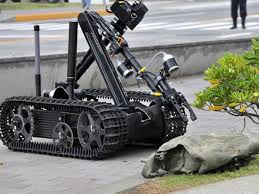
\includegraphics[width=0.33\textwidth]{imag/IMG1.jpeg}}
  \subfloat[Robots en cadena de montaje]{
   \label{f:Robots en serie de montaje}
    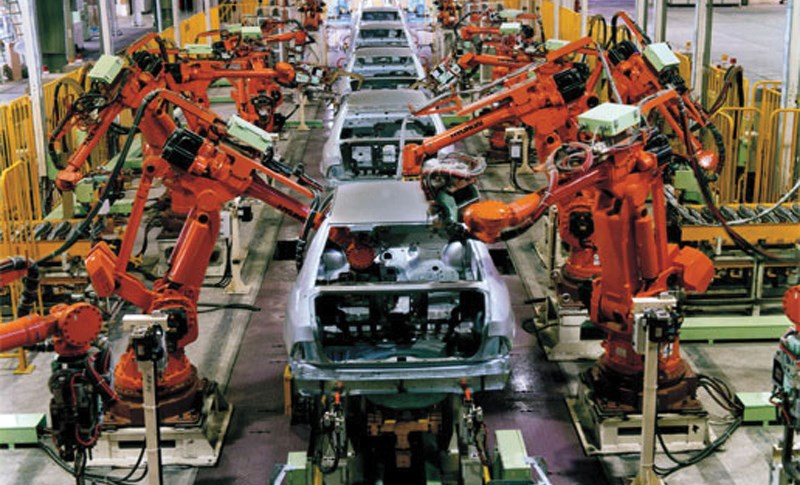
\includegraphics[width=0.33\textwidth]{imag/IMG2.jpeg}} 
  \subfloat[Rover Curiosity en Marte]{
   \newline\label{f:Rover Curiosity en Marte}
    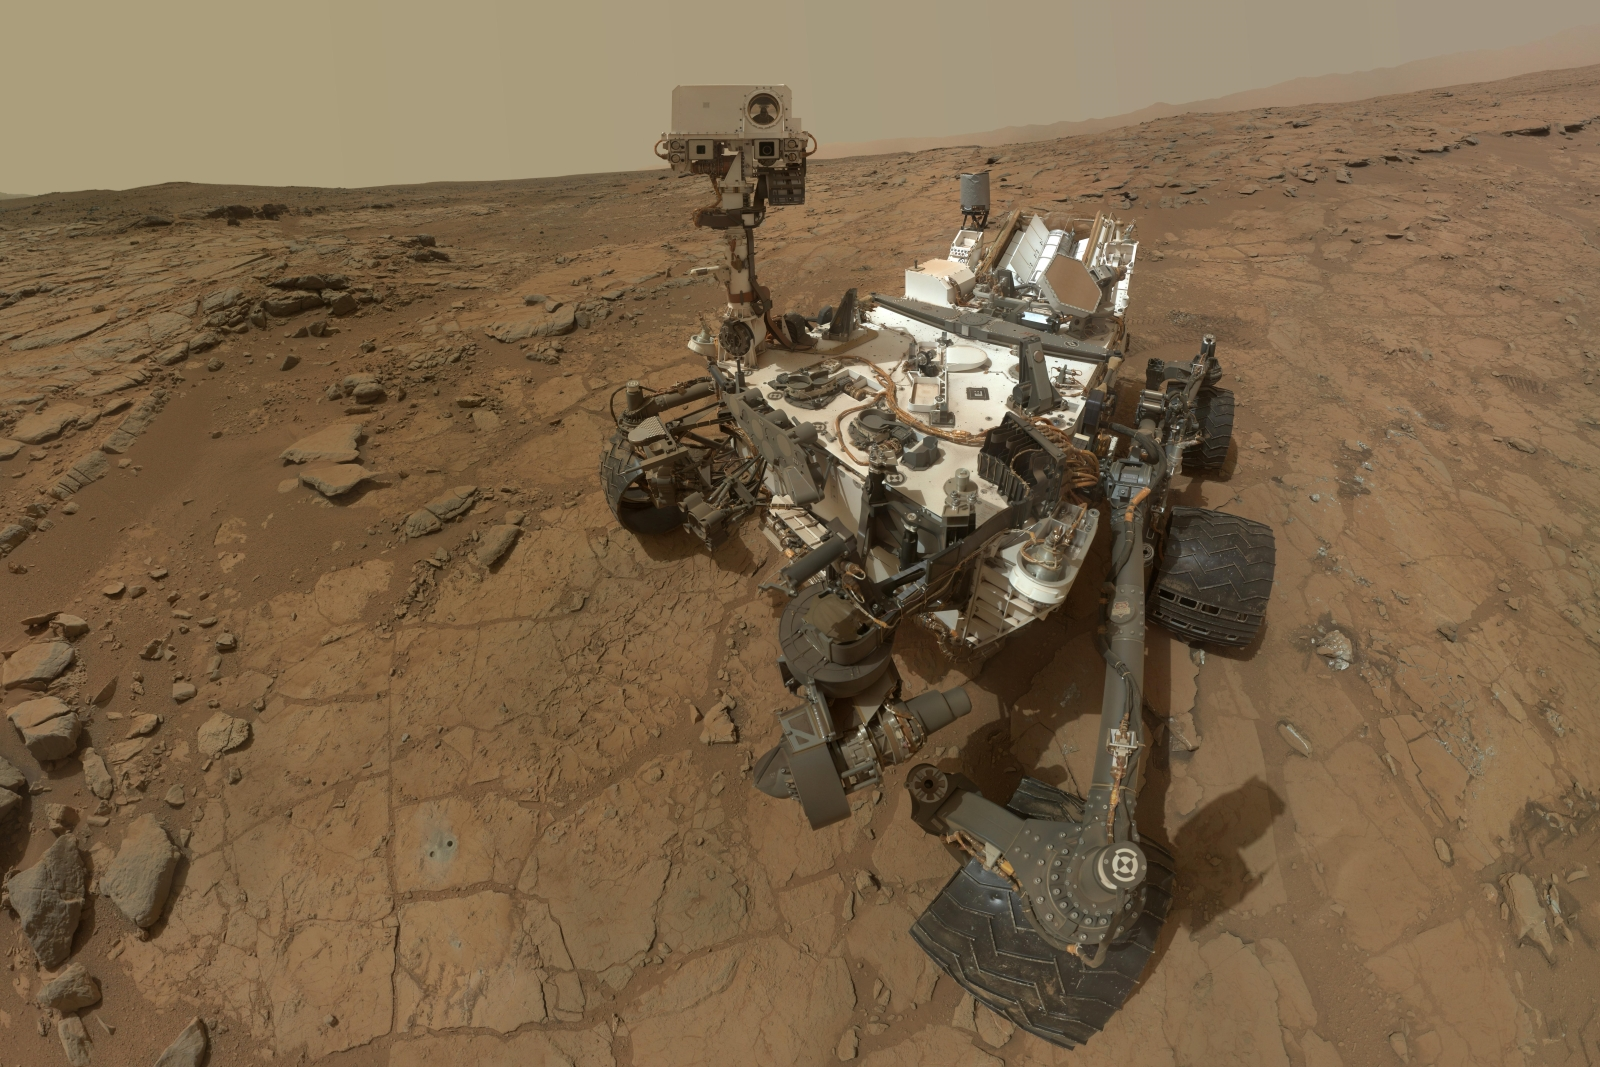
\includegraphics[width=0.33\textwidth]{imag/IMG3.jpeg}} 
 \caption{Ejemplos de funcionalidades de robots}
 \label{f:Ejemplos de funcionalidades de robots}
\end{figure}  

\subsection{Clasificación}
\hspace{1cm} Hay muchas clasificaciones posibles de los robots, uno, bastante utilizado, y reconocido, es según su cronología:

\begin{itemize}
		\item \textbf{1ª Generación:} Robots manipuladores. Sistemas mecánicos de varias funcionalidades con un sistema de control sencillo, el cual puede ser manual, de secuencia fija o de secuencia variable.

	\item\textbf{2ª Generación:} Robots de aprendizaje. Son capaces de repetir una secuencia de movimiento que ha sido previamente ejecutada por una persona. El operador realiza los movimientos requeridos mientras el robot los memoriza y le va siguiendo. 

	\item\textbf{3ª Generación:} Robots con control sensorizado. Llevan incorporados controladores, pequeñas computadoras que ejecutan las órdenes de un programa y es capaz de realizar los movimientos ordenados.

	\item\textbf{4ª Generación:} Robots inteligentes. Similares a la generación anterior pero incluyen una gran mejora, están equipados con sensores que mediante la comunicación con la computadora de control permite una toma inteligente de decisiones y un control de procesos en tiempo real.
\end{itemize}

\begin{figure}[H]
	\begin{center}
		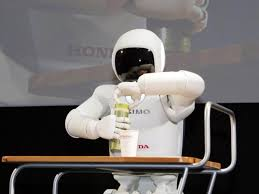
\includegraphics[width=0.5\textwidth]{imag/IMG11.jpeg}
				\caption{Robot ASIMO realizando acciones cotidianas.} 
	\label{fig:Robot ASIMO.}	
	\end{center}
\end{figure}

\subsection{Aplicaciones}
\hspace{1cm} La robótica está en constante desarrollo, esto ligado al incremento de los procesadores, así como en dispositivos hardware y desarrollo de software ha permitido que la robótica esté presente en prácticamente todas las industrias actuales y cotidianas de nuestra vida:
\begin{itemize}
		\item \textbf{Agricultura: }Hoy en día es muy común ver robots que controlen y monitorice por sí solos las cosechas y a medida que pasa el tiempo se vuelven más y más populares. La tecnología robótica aplicada al sector agrícola se encuentra en un estado de desarrollo avanzado debido a la necesidad de aumentar la producción sin aumentar los recursos, al mismo tiempo que se minimiza el impacto ambiental.
		\item \textbf{Educación: }La robótica ha surgido como un recurso didáctico innovador que favorece la enseñanza de conceptos y conocimientos de distintas disciplinas, no únicamente las tecnológicas o científicas.  Además, esta tecnología  se utiliza como factor de motivación, a partir del interés de los niños, para llevar al alumno al desarrollo de su propio conocimiento.
\\
		\begin{figure}[H]
			\begin{center}
				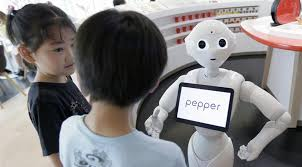
\includegraphics[width=0.9\textwidth]{imag/IMG12.jpeg}
					\caption{Robot PEPPER en un aula como complemento educador.}
			\label{fig:Robot PEPPER.}	
			\end{center}
		\end{figure}

		\item \textbf{Industria: }Se utilizan para realizar trabajos peligrosos o de gran dificultad para un humano, como puede ser la aplicación de sustancias nocivas, el moldeado de materiales o el transporte pesado; también para tareas de inspección y control de calidad mediante visión artificial y sistemas mecánicos. Además, el uso de robots conlleva una mejora de calidad y un gran aumento de la productividad, por ejemplo ayudando a la logística y el procesado final para los envíos.
		\item \textbf{Automovilismo: }En las fábricas se utilizan para ayudar en la fabricación, como los brazos robóticos de montaje o para el transporte de materiales, como los AGVs que son capaces de guiarse por la fábrica autónomamente. Fuera de éstas podemos observar vehículos con conducción autónoma que poco a poco son cada vez más utilizados, como Tesla, BMW y los sistemas de aparcamiento autónomo. También en la investigación espacial se hace un gran uso de la robótica, lo que permite investigar entornos que para un ser humano serían prácticamente imposibles, como el caso del robot Curiosity.
		\item \textbf{Medicina: }Se han desarrollado dispositivos que permiten realizar desde trabajos quirúrgicos guiados por imágenes hasta cirugía mínimamente invasiva realizada mecánicamente por un robot. Es el caso del robot DaVinci, capaz de realizar operaciones por sí solo con un nivel de precisión imposible de alcanzar por un humano y una gran velocidad. También podemos encontrar robots asistenciales para personas que necesitan una supervisión y cuidado continuo, prótesis robóticas para sustitución parcial de alguna parte dañada del cuerpo, o incluso exoesqueletos. Otro ejemplo estaría en la robótica terapéutica, utilizada como medio de rehabilitación fisiológica y de estimulación cognitiva en tratamientos para enfermedades como el Alzheimer.
		
		\begin{figure}[H]
			\begin{center}
				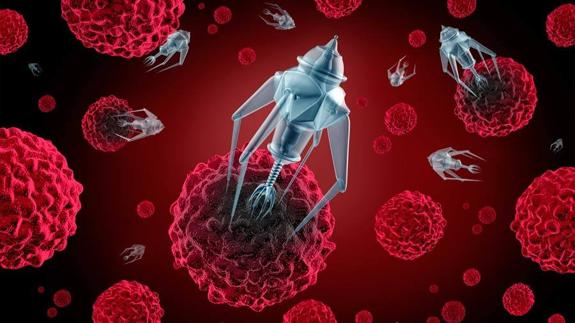
\includegraphics[width=0.54\textwidth]{imag/IMG13.jpeg}
					\caption{Robot DaVinci utilizado en hospitales.}
			\label{fig:Robot DaVinci.}	
			\end{center}
		\end{figure}	
			
		\item \textbf{Militar: } Actualmente existe una gran gama de vehículos terrestres sin piloto humano con funciones de reconocimiento e incluso algunos vehículos armados. Un ejemplo de esto sería el robot PackBot que según el medio en el que se encuentre se puede equipar con diferentes instrumentos para adaptarse a el. El mayor desarrollo en cuanto a robótica militar está siendo en la robótica aérea, donde estos sistemas han pasado de ser unidades de apoyo a unidades primarias de ataque.
		\item \textbf{Ocio y tiempo libre: }En los últimos años se ha producido una integración de esta tecnología en eventos de cultura, deporte y ocio e incluso en las casas. En las casas donde podemos ver robots autónomos que se encargan de las tareas domésticas como la aspiradora Roomba. Aquí también podríamos incluir los robots para niños que son capaces de divertir y entretener a la vez, y están llegando a todos los hogares, los más vendidos son los robots de LEGO donde los niños pueden aprender a crear robots y programarlos de una forma muy sencilla. Por último mencionaremos el robot que está creando gran expectación por sus habilidades locomotrices y aspecto humanoide, es el llamado Atlas creado por Boston Dynamics, capaz de correr y saltar en cualquier tipo de entorno e incluso de dar volteretas.
				
		\begin{figure}[H]
			\begin{center}
				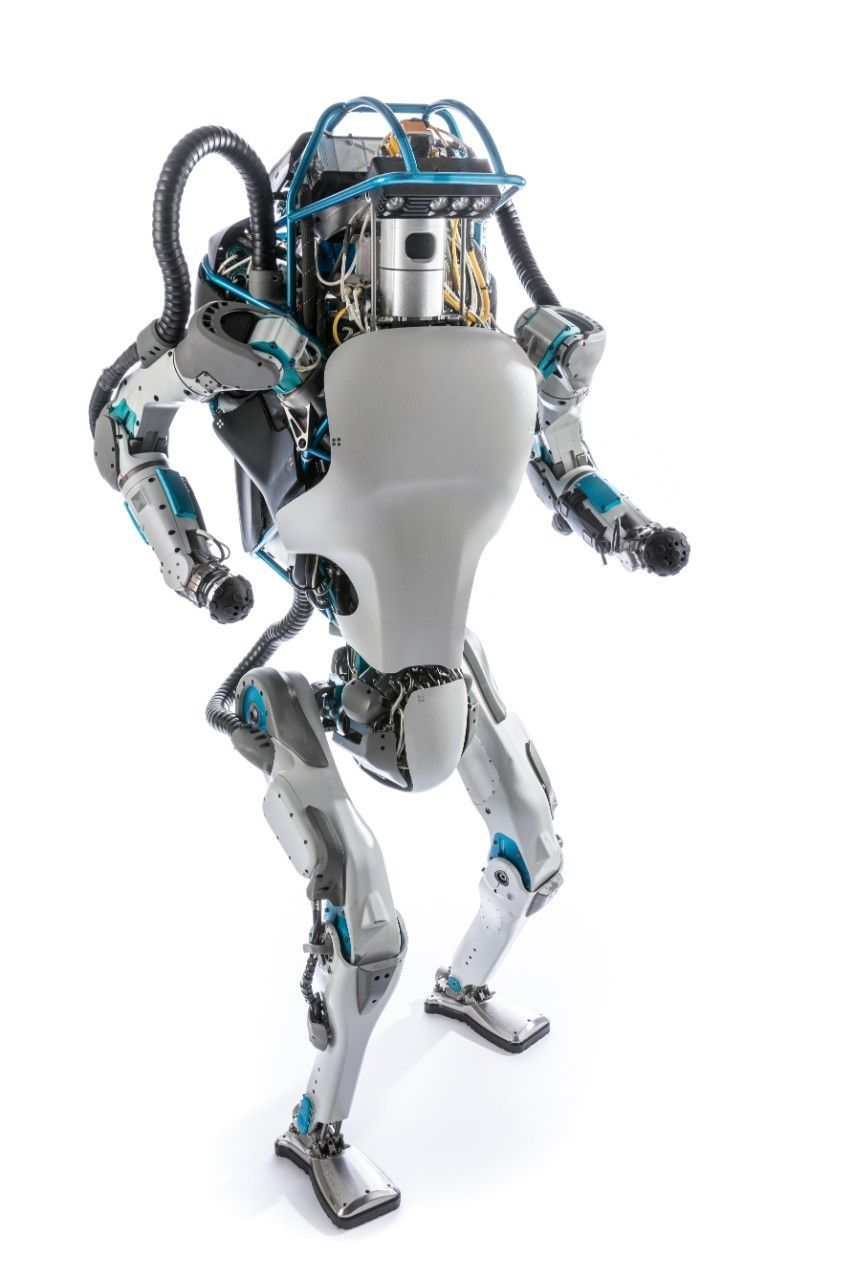
\includegraphics[width=0.25\textwidth]{imag/IMG29.jpg}
					\caption{Robot Atlas de aspecto humanoide.}
			\label{fig:Robot Atlas.}	
			\end{center}
		\end{figure}
		
		\item \textbf{Seguridad: }La robótica ha dado al mundo de la seguridad y la vigilancia una nueva perspectiva, siendo la visión artificial el eje en torno al que giran estas aplicaciones. La automatización de estas tareas permite una mayor facilidad y eficiencia a la hora de ejecutar esta labor, podemos encontrar drones que vigilan grandes concentraciones de personas, cámaras en seguridad vial que analizan el tráfico o el uso doméstico de estas para la prevención de accidentes.
\end{itemize}

\section{Robótica Aérea}
\hspace{1cm} Los robots aéreos, también conocidos como UAV (\textit{Unmanned Aerial Vehicle}), son vehículos aéreos no tripulados (VANT) controlados remotamente desde una estación de control en tierra y/o mar, o por un programa previamente implementado. Estos últimos son los llamados UAV autónomos, programados para que respondan ante el entorno e incluso interactúen con el.

\hspace{1cm} Inicialmente estos robots se pensaron únicamente para uso militar y fueron desarrollados por este sector. Empezaron a crearse entre los años 1914 y 1918, durante la I Guerra Mundial, como blancos aéreos de entrenamiento y defensa contra los Zeppelins. Se continuaron desarrollando durante la II Guerra Mundial también para entrenar a los operarios de los cañones antiaéreos. Pero pronto se vio el potencial que tenían estos robots aéreos y se empezó a utilizar también con fines más productivos como la vigilancia, iniciada durante la guerra de Vietnam,  y la obtención, manejo y transmisión de información ya sea propia u obtenida por los mismos UAV y así proteger la misma de la guerra electrónica y la criptografía ya que las comunicaciones son mucho más seguras y difíciles de detectar.

\hspace{1cm} Si bien el uso principal en el siglo XX era en la industria militar, en el siglo XXI visto el gran potencial que tenían, los nuevos usos que se les estaban dando y los avances en  la industria aeronáutica e informática hicieron que se convirtiese en una herramienta útil para la sociedad civil. En la actualidad los UAV son útiles en diferentes industrias con diferentes objetivos. Una posible clasificación de los usos de robots aéreos sería:

\begin{itemize}
		\item \textbf{Blanco:} Servían como simulación de aviones y ataque enemigos para entrenar las defensas de los ejércitos.
		\item\textbf{Reconocimiento:} Uso que reveló el gran potencial de estos robots, servían para enviar información militar recopilada durante el vuelo, normalmente en las zonas enemigas. 
	\begin{figure}[H]
		\begin{center}
			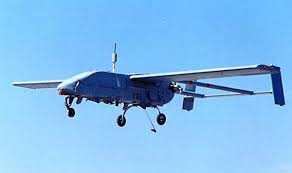
\includegraphics[width=0.7\textwidth]{imag/IMG14.jpeg}
					\caption{AAI RQ-2 Pioneer - Uno de los primeros Robots Aéreos.}
		\label{fig:UAV Pioneer.}	
		\end{center}
	\end{figure}		
		
		\item \textbf{Combate:} estos son los llamados UCAV(\textit{unmanned combat air vehicle}) usados para llevar a cabo misiones de combate que suelen ser peligrosas.
		\item \textbf{Logística:} o también llamados de carga, utilizados sobretodo para transportar mercancías peligrosas o sobre zonas en conflicto sin el riesgo de perder vidas humanas.
		\item \textbf{Investigación y Desarrollo:} en éstos se exploran, prueban y mejoran los sistemas que avanzan cómo serán los drones del futuro.
		\item \textbf{Comercial y Civil:} esta utilización se encuentra en enorme crecimiento tanto de innovaciones como de ventas ya que son diseñados para propósitos civiles como: realizar filmaciones , inspección y reparaciones, sondas de investigación, rescates, vigilancia, detección de incendios y agricultura entre otros.
\end{itemize}

\subsection{Componentes}
\hspace{1cm} La mayoría de los UAV actuales cuentan con una serie de partes, sensores y actuadores que les permiten realizar los propósitos para los que has sido creados, entre ellos se encuentran: 
	\begin{itemize}
		\item \textbf{Motor:} En cuanto a la disposición de los motores diferenciaremos los de ala fija los cuales se rigen por el mismo principio de vuelo que los aviones en los cuales la sustentación se produce gracias a la forma de las alas y el enfrentamiento de estas frente al viento, y los de ala rotatoria, donde los motores giran en horizontal, estos se rigen por el principio de vuelo de los helicópteros en los cuales las propias hélices del motor son las que por su forma y giro producen la sustentación y el vuelo del drone.
		 		
\begin{figure}[H]
 \centering
    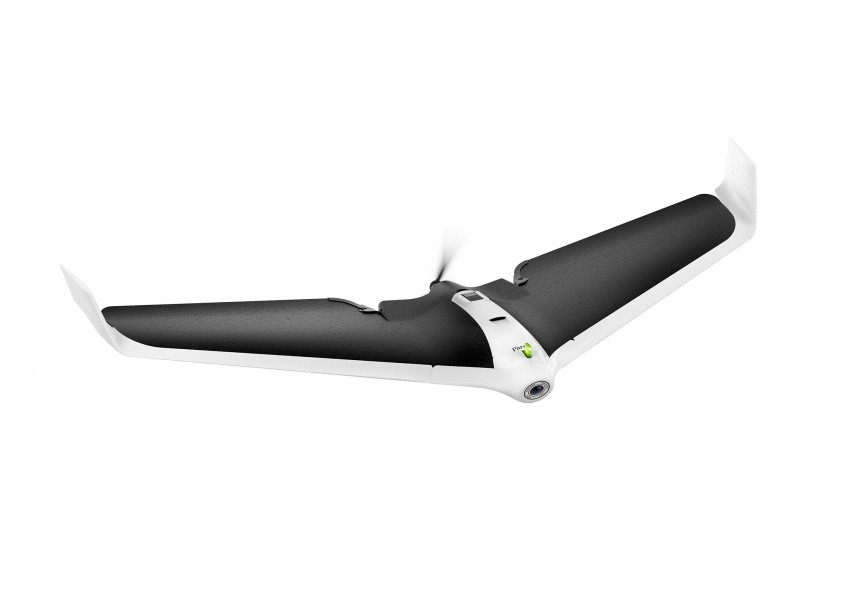
\includegraphics[width=7cm,height=4cm]{imag/IMG15.jpeg}
    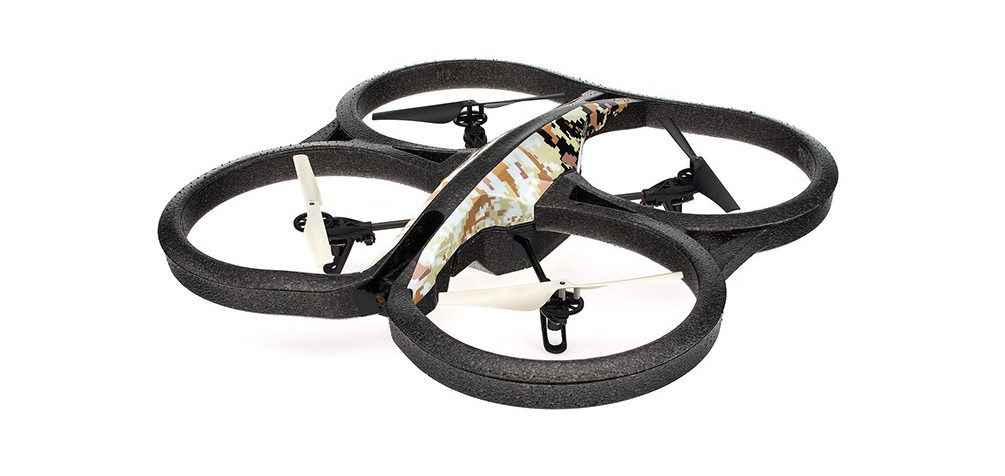
\includegraphics[width=7cm,height=4cm]{imag/IMG16.jpeg}
 \caption{Drone ala fija Vs Drone ala móvil}
 \label{f:Tipos de Drone}
\end{figure}

		\item \textbf{Chasis:} Estructura principal  sobre  la  que  se sitúan el resto de los elementos. Cambiará su forma dependiendo del tipo de UAV, variando la longitud del cuerpo de aterrizaje o el número de soportes para los motores o hélices. Gracias a los últimos avances en la ingeniería de materiales se ha conseguido que el chasis sea muy ligero y con ello incrementar la carga útil (\textit{pay-load}) para mejorar la funcionalidad de los mismos.
		\item \textbf{Batería:} La parte más crítica de los UAV actualmente y en la que más se está investigando. La autonomía media de los UAV no supera la hora de vuelo y esto es debido a que los motores necesitan mucha potencia para poder volar los drones. Cuanto más grande es el drone más potencia es necesaria y por tanto mayor batería se necesita, por lo que hay que encontrar el equilibrio justo que se necesita para cada drone en cuanto a peso, carga útil y autonomía. 
		\item \textbf{Equipo transmisor y receptor:} Parte encargada la transformación de la información y, si fuese el caso, de la comunicación simultánea con el equipo en tierra. Es una parte muy importante para los UAV que están teledirigidos o que transmiten información simultánea de lo que están haciendo, normalmente mediante radiofrecuencia o Wi-Fi.
		\item \textbf{Controlador:} Encargado de recoger toda la información, tanto de la previamente cargada como de los sensores, para procesarla y de ejecutar las órdenes adecuadas para completar el objetivo que se le ha establecido. 
		\item \textbf{Cámara:} Aunque no todos los UAV la llevan incorporada, es una parte imprescindible en el desarrollo de los mismos ya que permite saber en todo momento lo que está realizando el drone y analizar estas imágenes para comprobar el correcto funcionamiento.
		\item \textbf{Altímetro:} Es el sensor que mide los cambios en la presión atmosférica de forma que puede establecer la altura a la que se encuentra el drone.
		\item \textbf{IMU:} es un dispositivo electrónico que mediante una combinación de acelerómetros y giróscopos determina la velocidad, orientación y las fuerzas gravitacionales del vehículo.
		\item \textbf{Magnetómetro:} es un dispositivo que mide la dirección del campo gravitacional de la tierra y de esta forma calcula la orientación del dispositivo con respecto a ésta, lo cual es muy útil para direccionar el drone sobre rutas terrestres.
	\end{itemize}

\subsection{Movimiento de cuadricópteros}
\hspace{1cm} En este TFG nos centraremos sobretodo en los Robots Aéreos de ala móvil, concretamente en los cuadricópteros, que son los que están formados por cuatro hélices las cuales permiten el movimiento en todas las direcciones posibles mediante la variación de potencia de los motores que hacen girar estas hélices. En la imagen \ref{f:Moviento en drones.} se pueden observan cómo se producen los principales movimientos del drone. Las flechas indican el sentido de rotación de las hélices y el color la velocidad del giro, el rojo significa mayor velocidad. Como diferenciación de la forma de vuelo de los helicópteros destacar que en éstos la torsión generada por el rotor principal se contrarresta con una hélice de apoyo perpendicular a ésta y en los drones cuadricópteros el problema de la torsión se solventa asignando el sentido de giro de las hélices de forma opuesta entre rotores que están situados de forma contigua.

\begin{figure}[H]
 \centering
  \subfloat[Rotores en cruz +]{
   \label{f:Rotores en cruz}
    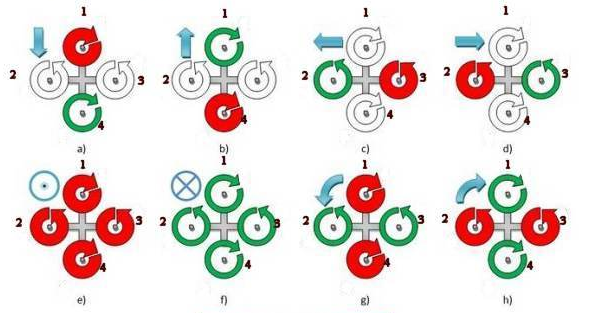
\includegraphics[width=0.53\textwidth]{imag/IMG5.png}}
  \subfloat[Rotores en aspa x]{
   \label{f:Rotores en aspa}
    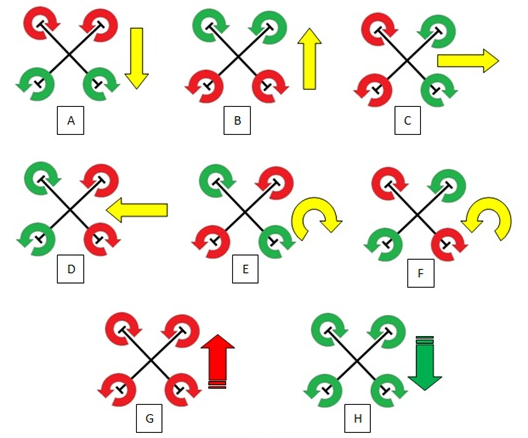
\includegraphics[width=0.38\textwidth]{imag/IMG6.png}} 
 \caption{Movimiento del Drone según sus rotores.}
 \label{f:Moviento en drones.}
\end{figure}

\subsection{Marco legislativo español para drones}
\hspace{1cm} En el marco legislativo actual en España sobre los UAV se acordó el 15 de Diciembre de 2017 en el Consejo de Ministros y se publicó en el BOE \cite{BOE}. La nueva ley sigue cumpliendo prácticamente la totalidad de la ley aprobada el 4 de Julio de 2014 en la cual se especificaba: 
\begin{itemize}
		\item Tipo de Drone: Se establecen dos categorías iniciales: Drones con peso inferior a 2Kg. y drones con peso entre los 2Kg. y 25Kg. Para operar cualquiera de ellos es imprescindible disponer de un carnet de piloto de drones válido en toda España. En caso de los drones de peso inferior a 2kg, no será necesario que estén inscritos en el registro de aeronaves ni disponer de un certificado de aeronavegabilidad. Para ambos tipos de drone será necesario incluir obligatoriamente una placa identificativa con el nombre del fabricante del aparato así como los datos fiscales de la empresa que lleve a cabo dichas operaciones.
		\item Espacio aéreo: El espacio aéreo pertenece a AESA, y como tal, para poder realizar cualquier tipo de actividad comercial o civil con un drone, se deberá obtener un permiso oficial, como mínimo 5 días antes de llevar a cabo cualquier operación en el aire. Esta nueva legislación sigue manteniendo la prohibición de sobrevolar núcleos urbanos o espacios con una alta masificación de gente sin el consentimiento especial por parte de la Agencia Española de Seguridad Aérea.
		\item Seguridad: El pilar fundamental en el que se ha basado el Ministerio para la realización de la normativa de uso de drones civiles en España es la seguridad. Por ello cada empresa deberá disponer de un manual de operaciones cumplimentado siguiendo el estándar proporcionado por el Ministerio, así como un estudio de seguridad de cada una de las operaciones a realizar. Es decir, si alguien piensa en hacer volar un drone al margen de la ley, ya sea con un peso inferior a 2kg, o entre 2kg y 25kg, se expone a sanciones que van entre 3.000\textup{\euro} a 60.000\textup{\euro}.
		\item Carnet de piloto de Drones en España: Para que las empresas puedan operar legalmente los pilotos designados deberán disponer de un carnet oficial para el manejo de drones. Si estos pilotos ya disponen de un título de piloto de avión, ultraligero u otro específico, no será necesario obtener dicha titulación. En caso contrario deberán cursar una serie de exámenes y pruebas oficiales para obtener el carnet oficial de piloto de drones. A día de hoy, no existen academias oficiales bajo la tutela del Gobierno que realicen estos cursos, por eso y mientras se empiezan a impartir estos cursos, será obligatorio demostrar que se dispone de los conocimientos teóricos y algún tipo de carnet oficial o documento que acredite a los pilotos en el manejo de drones para poder llevar a cabo cualquier operación. Esta normativa temporal sobre drones en España considera los diferentes marcos en los que se podrán realizar los distintos trabajos aéreos en función del peso de la aeronave. Además, el texto aprobado se completa con el régimen general de la Ley 48/1960, de 21 de julio, sobre Navegación Aérea, y no sólo marca las pautas de operación con este tipo de aeronaves, sino también otro tipo de obligaciones.
	\end{itemize}
	
\hspace{-1cm} Las únicas novedades de la ley puesta en marcha a finales del año pasado son:

	\begin{itemize}
		\item Sobrevolar zonas pobladas: Ésta es una de las medidas más esperadas por el sector. Se podrán realizar vuelos sobre aglomeraciones, edificios y reuniones de personal al aire libre siempre y cuando la masa máxima al despegue de la aeronave no sobrepase los 10kg, mantengamos la aeronave dentro del alcance visual del piloto (VLOS) y no sobrepasemos los 120 metros de altura ni los 100 metros en horizontal con la posición del piloto.
		\item Vuelos en espacio aéreo controlado: Por el momento sólamente está permitido volar en zonas de espacio aéreo no controlado. Con la nueva ley se podrá volar en espacio aéreo controlado siempre y cuando presentemos los estudios de seguridad correspondiente y tengamos la autorización de AESA.
		\item Operaciones EVLOS: Con la normativa vigente solamente podemos alejar nuestra aeronave a una distancia máxima de 500 metros en horizontal respecto a la posición del piloto. Con la nueva normativa estarán permitidos los vuelos dentro del alcance visual aumentado (EVLOS). Es decir, estos 500 metros pueden ser ampliados, siempre y cuando existan observadores intermedios coordinados entre si. En todo momento, al menos uno de ellos debe tener visión directa del vehículo.
	\end{itemize}	 

\subsection{Competiciones con robots aéreos}
\hspace{1cm} En cuanto a los inventos de drones o de usos de éstos ilustraremos tres certámenes importantes. A nivel internacional tenemos el Premio \textit{UAE Drones For Good Award} en los Emiratos Árabes en el cual los siguientes proyectos españoles han llegado a ser finalistas: transferir rápidamente órganos de trasplantes desde los centros de donantes, vigilar mejor las zonas verdes para combatir la caza furtiva, controlar la vida salvaje y reducir el riesgo se incendios, ofrecer mejor detección de campo de minas y combatir la propagación de la enfermedad del sueño (Tse-Tse) mediante el control de mosquitos.

\hspace{1cm} El \textit{UAV Challenge - Outback Rescue} presenta un desafío abierto para adultos y un desafío para la escuela secundaria. El evento tiene como objetivo promover el uso civil de vehículos aéreos no tripulados y el desarrollo de sistemas de bajo costo que podrían usarse para misiones de búsqueda y rescate. Es uno de los desafíos de robótica más grandes del mundo y uno de los desafíos de UAV de mayor riesgo, el premio para el ganador es de 75.000 \$.

\begin{figure}[H]
	\begin{center}
		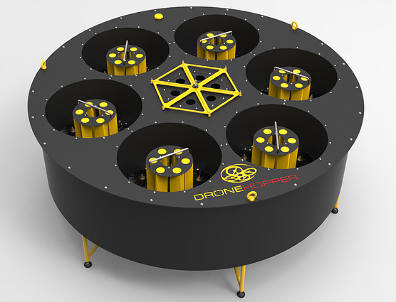
\includegraphics[width=0.7\textwidth]{imag/IMG7.jpeg}
				\caption{Dron contra incendios.} 
	\label{fig:Dron Hopper.}	
	\end{center}
\end{figure}

\hspace{1cm} A nivel nacional tenemos el Premio que se ha creado este año a la Innovación Aeronáutica por el COIAE(Colegio Oficial de Ingenieros Aeronáuticos de España) y que ha ganado, drone que extingue incendios forestales, el cual tiene la capacidad de adaptarse a las condiciones de un fuego para apagarlo\footnote{\url{https://www.drone-hopper.com}}.


\section{Visión Artificial y Autolocalización}
\hspace{1cm}  El drone manejado en este TFG incorpora un sistema de autolocalización visual, para muchos científicos el sentido del cual el ser humano obtiene más información del medio es la visión. De hecho, debido a esta gran cantidad de datos se estima que el 70\% de las tareas del celebro se emplean en analizar estos datos visuales. La Visión Artificial o Visión por Computador busca extraer la información visual desde los datos visuales mediante procedimientos automáticos. Para conseguir que esto sea viable y no se tarde días se han desarrollado técnicas de procesamiento de imágenes que han avanzado a niveles de que el desfase entre la visión artificial y la realidad sea prácticamente nulo.

\begin{figure}[H]
	\begin{center}
		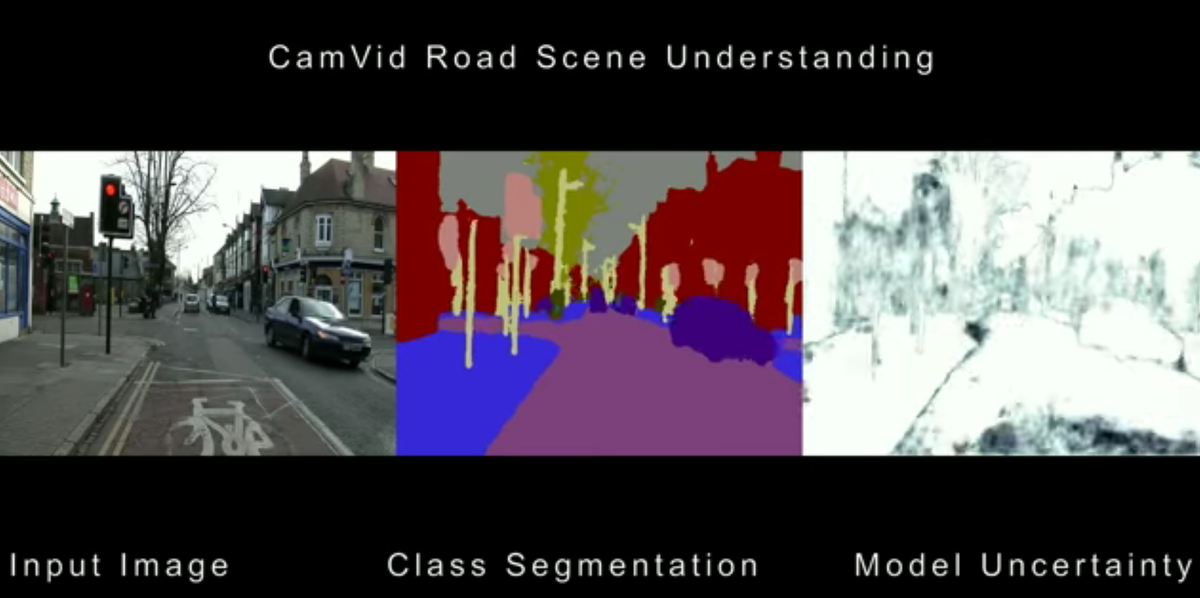
\includegraphics[width=0.9\textwidth]{imag/IMG4.png}
				\caption{Visión artificial de un automóvil.}
	\label{fig:Vista artificial automoviles.}	
	\end{center}
\end{figure}

\hspace{1cm} La visión artificial se basa en la naturaleza de la luz, que es la parte de la radiación electromagnética que puede ser percibida por el ojo humano, está formada por fotones cuyas propiedades en relación con la dualidad de onda explican las características de su comportamiento. La Visión Artificial se basa en la formación de imágenes y, como hemos dicho antes, en el sistema de procesamiento de éstas. Típicamente el primer apartado de un sistema de visión artificial estaría constituido  por  el  subsistema  de  iluminación,  de  captación  de  la  imagen  y  de adquisición  de  la  señal  en  el  computador. Una vez se ha conseguido introducir la señal en el computador se procesa mediante algoritmos para transformarla en información útil para los robots.

\hspace{1cm} En estos últimos años y gracias a la privatización del GNSS y la utilización de este sistema para la sociedad, ha permitido que hoy podamos utilizar la localización en cualquier dispositivo con una simple antena, a su vez y visto el potencial de este sistema de autolocalización todos los países han intentado crear su red satelital de posicionamiento, el primero y promotor de todo fue GPS (EE.UU.), además existen Galileo (UE), Beidu (India), Glonass (Rusia)... Con toda esta red de satélites y la posibilidad de los nuevos softwares que permiten la utilización de varios sistemas conjuntamente todos los nuevos dispositivos utilizan un localizador GNSS, el problema ocurre cuando la posición que necesitamos es tridimensional y tiene que ser muy precisa, ya que este sistema aun cuenta con fallos de metros en cuanto al posicionamiento tridimensional. Por ello, en nuestro proyecto, no podremos utilizar este sistema de posicionamiento y lo cambiaremos por un sistema de autolocalización basado en visión y en balizas, el cual nos dará un error mucho menor y nos permitirá realizar el enrutamiento y guiado mucho más preciso.
\\
\\
\\
\\

\section{Robótica aérea con JdeRobot}
\hspace{1cm} Este TFG se enmarca en el ecosistema del proyecto de software libre para robots JdeRobot. Los antecedentes inmediatos a este TFG en los que me he basado y que me han ayudado para crear mi trabajo han sido:

\hspace{1cm} Alberto Martín \footnote{\url{http://jderobot.org/Amartinflorido-tfm}} \cite{AlbertoMartin} \textit{Navegación visual en un cuadricóptero para el seguimiento de objetos.} En él abordaba la navegación visual autónoma de un cuadricóptero implementando algoritmos de navegación visual para el seguimiento de objetos de manera automática tanto utilizando la cámara frontal como utilizando la cámara inferior.
\\

\begin{figure}[H]
	\begin{center}
		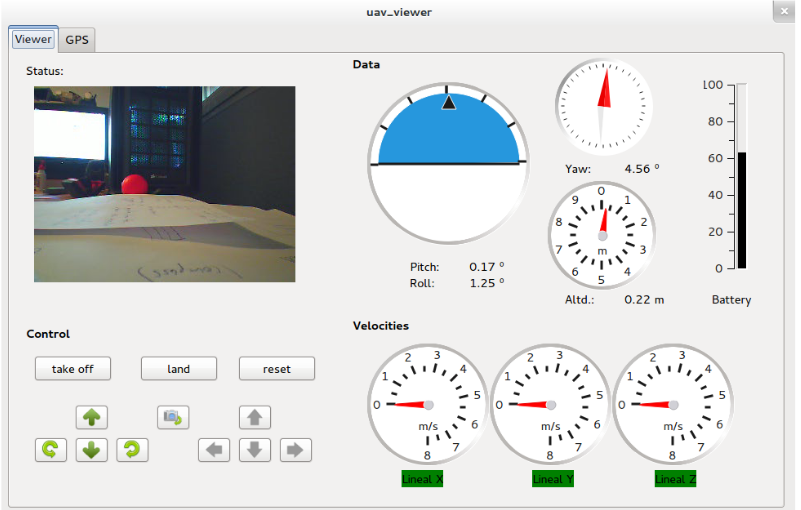
\includegraphics[width=0.7\textwidth]{imag/IMG8.png}
				\caption{TFM Alberto Martín.} 
	\label{fig:TFM Alberto M.}	
	\end{center}
\end{figure}

\hspace{1cm} Daniel Yagüe  \footnote{\url{http://jderobot.org/Daniyague-pfc}} \cite{DanielYague} \textit{Cuadricóptero AR.Drone en Gazebo y JdeRobot}. En el cual su objetivo era proporcionar un soporte para robots aéreos dentro del simulador Gazebo en el entorno JdeRobot y crear varias aplicaciones de navegación para validarlo.
\\
\\

\hspace{1cm} Alberto López-Cerón \footnote{\url{http://jderobot.org/Alopezceron-tfm}} \cite{AlbertoLopez} \textit{Autolocalización visual robusta basada en marcadores.} Su objetivo principal era crear un algoritmo de autolocalización visual basado en marcadores, es decir, a partir de la detección de balizas estimar la posición de la cámara. Fue creado tanto para el entorno de simulación como para entornos reales.
\\

\hspace{1cm} Arturo Vélez \footnote{\url{http://jderobot.org/Avelez-tfg}} \cite{ArturoVelez} Dedicado al \textit{seguimiento de un objeto con textura desde un drone con cámara.} Aquí trabajó en un seguimiento visual, esta vez sin filtro de color, donde el drone sigue una textura en movimiento detectando unos puntos de interés para reconocerla.
\\

\hspace{1cm} Manuel Zafra \footnote{\url{http://jderobot.org/Mazafrav-pfc}} \cite{ManuelZafra} Centrado en el \textit{seguimiento de rutas 3D por un drone con autolocalización visual con balizas.} Diseñó un sistema de vuelo autónomo para drones en espacios interiores, basándose en la autolocalización mediante la visión artificial como se puede observar en la figura \ref{f:TFG Manuel Zafra}.
\\

\begin{figure}[H]
 \centering
    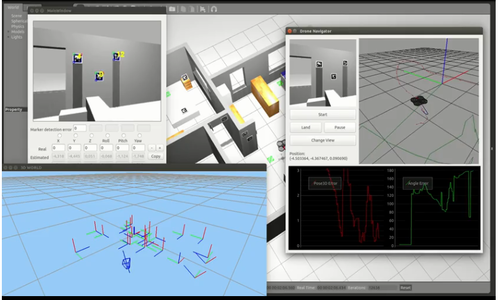
\includegraphics[width=7.5cm,height=6cm]{imag/IMG9.png}
    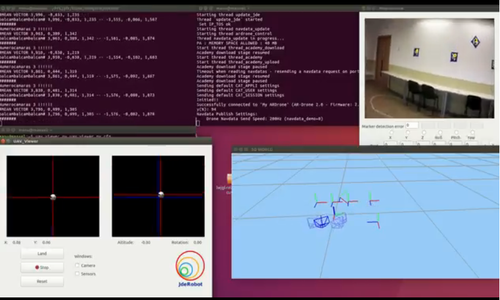
\includegraphics[width=7.5cm,height=6cm]{imag/IMG10.png}
 \caption{TFG Manuel Zafra.}
 \label{f:TFG Manuel Zafra}
\end{figure} 

\hspace{1cm} Jorge Vela \footnote{\url{http://jderobot.org/Jvela-tfg}} \cite{JorgeVela} Aborda el \textit{despegue, navegación y aterrizaje visuales de un drone usando JdeRobot.} Se centró en la localización y aterrizaje controlado por visión de un drone mediante la detección visual de balizas visible en la figura \ref{f:TFG Jorge Vela}.

\begin{figure}[H]
	\begin{center}
		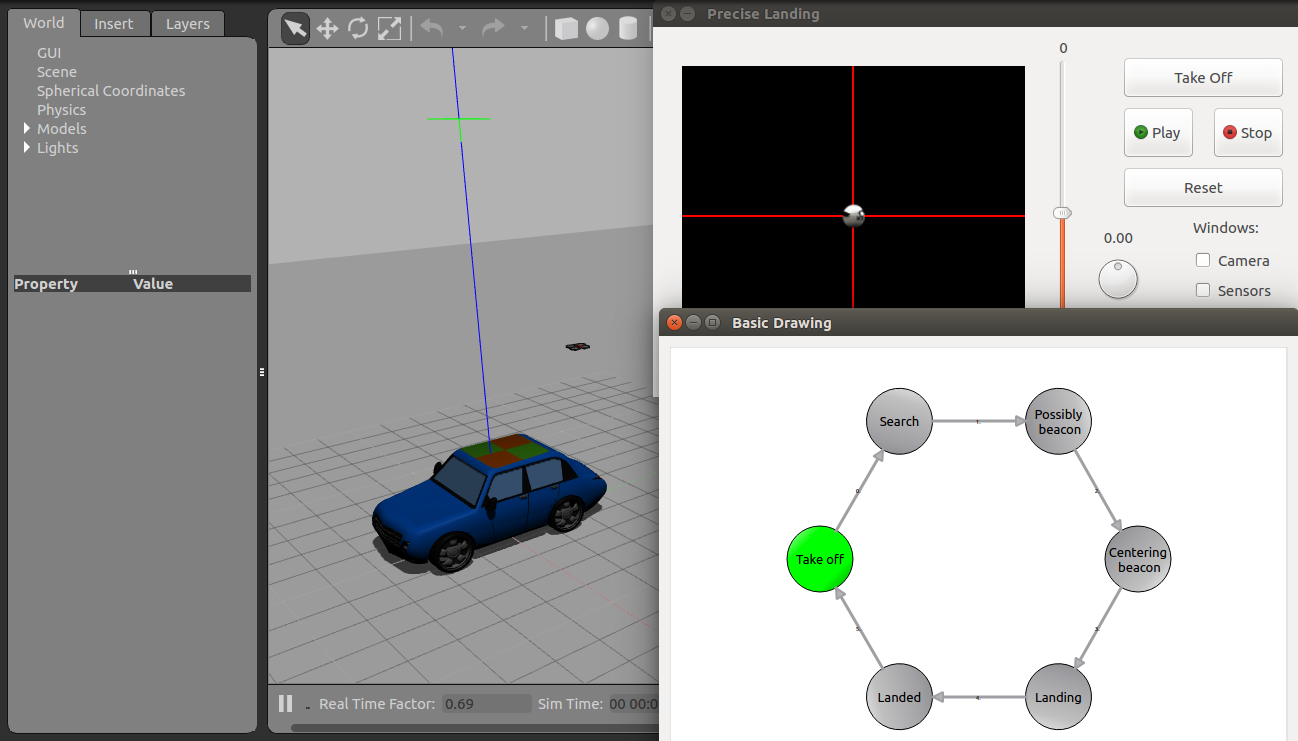
\includegraphics[width=0.8\textwidth]{imag/IMG50.png}
				\caption{TFG Jorge Vela.}
	\label{f:TFG Jorge Vela}	
	\end{center}
\end{figure}

\hspace{1cm} Una vez expuesta la breve introducción, el resto de la memoria se ha organizado en otros cinco capítulos. En el capítulo 2 se redactan los objetivos propuestos y la metodología seguida para llegar hasta ellos. En el capítulo 3 se presenta la infraestructura que hemos utilizado. En el capítulo 4 se describe el diseño y la implementación del algoritmo realizado, cómo se ha programado y cómo se ha integrado junto con los demás algoritmos en una sola aplicación final. En el capítulo 5 se detallan los distintos experimentos realizados, los resultados y los errores cuantificados que se han obtenido. Por último, en el capítulo 6 se incluyen las conclusiones a las que se han llegado tras finalizar este proyecto y los trabajos futuros que se podrían realizar.

%\lhead[]{CAPÍTULO \thechapter. OBJETIVOS}
\chapter{Objetivos}\label{cap.objetivos}
\hspace{1cm} Una vez introducidas las motivaciones que me han llevado a hacer este tfg y expuestos los conceptos mas importantes que se deben saber para comprender la totalidad del trabajo, en este capitulo se van a exponer los diferentes problemas que se abordaran a lo largo de la memoria, los requisitos para poder abordar estos problemas y por último la metodología y el plan de trabajo que se ha seguido. 


\section{Problemas a abordar}
\hspace{1cm} El objetivo principal de este trabajo es la creación de un sistema  que permita el funcionamiento de un dron completamente autónomo con esto queremos decir que despegue de forma controlada, siga una ruta previamente establecida y aterrice tambien de forma controlada. Para la parte de enrutamiento el drone ha de conocer en todo momento su posición en
el entorno mediante técnicas de visión por computador basadas en marcadores visuales
artificiales, mientras que para el despegue y aterrizaje controlados debe reconocer las balizas por visión cuya posición es desconocida. 

\hspace{1cm} Conociendo el objetivo principal este se ha desglosado en varios subobjetivos para poder abordarlo correctamente:

\begin{enumerate}
	\item{\textbf{Utilización de la herramienta Visual States:} La cual nos permitirá crear la jerarquía necesaria para poder pasar de un estado a otro mediante transiciones y así poder dividir nuestro programa e ir mejorándolo e implementando las nuevas creaciones sin tener que modificar las otras partes, además de esto creará una interfaz gráfica en la cual representa el comportamiento del robot gráficamente y así se puede distinguir el estado en el que se encuentra. Esta representación gráfica permite un mayor nivel de abstracción para el usuario, ya que solo tiene que preocuparse por programar las acciones actuales del robot y seleccionar qué componentes puede necesitar de la interfaz del robot.}
	\item{\textbf{Adaptación e integración del componente Slam-Visualmarkers:} Como nadie había utilizado la herramienta de Visual States integrando el componente de slam-visualmakers hemos tenido que ajustar este componente e introducirlo por pasos para poder finalmente conseguir su correcto funcionamiento en la misma.}
	\item{\textbf{Recodificación e integración del aterrizaje visual:} Ya que este estaba creado a partir de una posición dada en altura y contaba con temporizadores y una maquina virtual de estados. Por esto se ha modificado para poder integrarlo en nuestro sistema de navegación y además a partir de este se ha creado el propio sistema de despegue controlado.}
	\item{\textbf{Desarrollo de dos componentes de navegación basados en la posición absoluta del drone:} Ambos serán controles de pilotaje aplicados sobre las posiciones obtenidas por el componente slam-visualmarkers, la diferencia radicara en que a uno le estableceremos una serie de puntos o balizas a los cuales debe de llegar mientras que el otro deberá seguir una ruta.}
	\item{\textbf{Validación experimental en entorno simulado Gazebo:} Se creará un mundo tridimensional en el que se realizarán las pruebas pertinentes para determinar la robustez
del sistema en conjunto. Se examinará para ambos componentes de navegación el error de la estimación de posición y cómo este puede afectar al sistema de pilotaje del cuadricóptero, ademas se comparara con anteriores sistemas de pilotajes y se verán las posibles mejoras. También se calculará el error producido en la estimación de posición por el componenete Slam-Visualmakers.}
\end{enumerate}


\section{Requisitos}
\hspace{1cm} Una vez descritos todos los objetivos, lo siguiente es nombrar los requisitos que va a satisfacer la aplicación que hemos desarrollado:

\begin{itemize}
		\item El algoritmo funcionará en la plataforma de desarrollo JdeRobot-5.6.3.
		\item El sistema se ejecutara en el entorno GNU/Linux Ubuntu 16.04.
		\item La aplicación se ejecutara en el simulador Gazebo con la utilización del robot Ar.Drone.
		\item El sistema debe ser exportable a cualquier escenario que sea un espacio simulado controlado y contenga marcadores AprilTags con posiciones conocidas.
		\item Para la autolocalización, el sistema sólo puede depender de las imágenes servidas por la cámara del drone y utilizando el componente Slam-Visualmarkers.
		\item El control de navegación mediante el pilotaje debe ser suave para no perder los marcadores y balizas, pero tambien robusto, fluido y vivaz para que el drone se mueva de forma ágil y veloz por el entorno y sus rutas establecidas.
		\item Programado en Python 2.7.
\end{itemize}


\section{Metodología}
\hspace{1cm} Al tratarse de un trabajo de integración y desarrollo software el modelo de trabajo que se ha seguido ha sido el de desarrollo en espiral. Este modelo nos ha permitido trabajar de forma progresiva, es decir, empezando por las partes mas sencillas y a medida que las íbamos logrando ir avanzando hasta las mas complejas. Para ello la forma de conseguirlo fue mediante la marcación de hitos o pautas a alcanzar que se revisaban periódicamente mediante reuniones con el tutor, de esta forma se analizaban si se había conseguido llegar al resultado esperado en cada etapa y así poder pasar al siguiente objetivo analizando para ello las posibles rutas que se podían seguir según la toma de decisiones y la evaluación de riesgos. Cuando se alcanzaba un objetivo lo suficientemente importante se creaba una entrada en el cuaderno de bitácora de JdeRobot, el cual es público y nos ha servido para llevar un seguimiento de las áreas realizadas y como punto de comunicación con el tutor para saber las dificultades que teníamos y como poder solucionarlas.  

\hspace{1cm} En el siguiente enlace del mediawiki o cuaderno de bitácora mencionado anteriormente se pueden encontrar desde fotos y videos de la practica final como resultados y pasos iniciales que se hicieron para adentrarse en el mundo de la programación de robots y drones \href{http://jderobot.org/Jsaizc-tfg}{http://jderobot.org/Jsaizc-tfg}. Tambien se puede visitar el código de todas estas etapas que se observan en el mediawiki, este es de acceso público en GitHub \href{https://github.com/RoboticsURJC-students/2017-tfg-jesus-saiz}{https://github.com/RoboticsURJC-students/2017-tfg-jesus-saiz}.

\begin{figure}[H]
	\begin{center}
		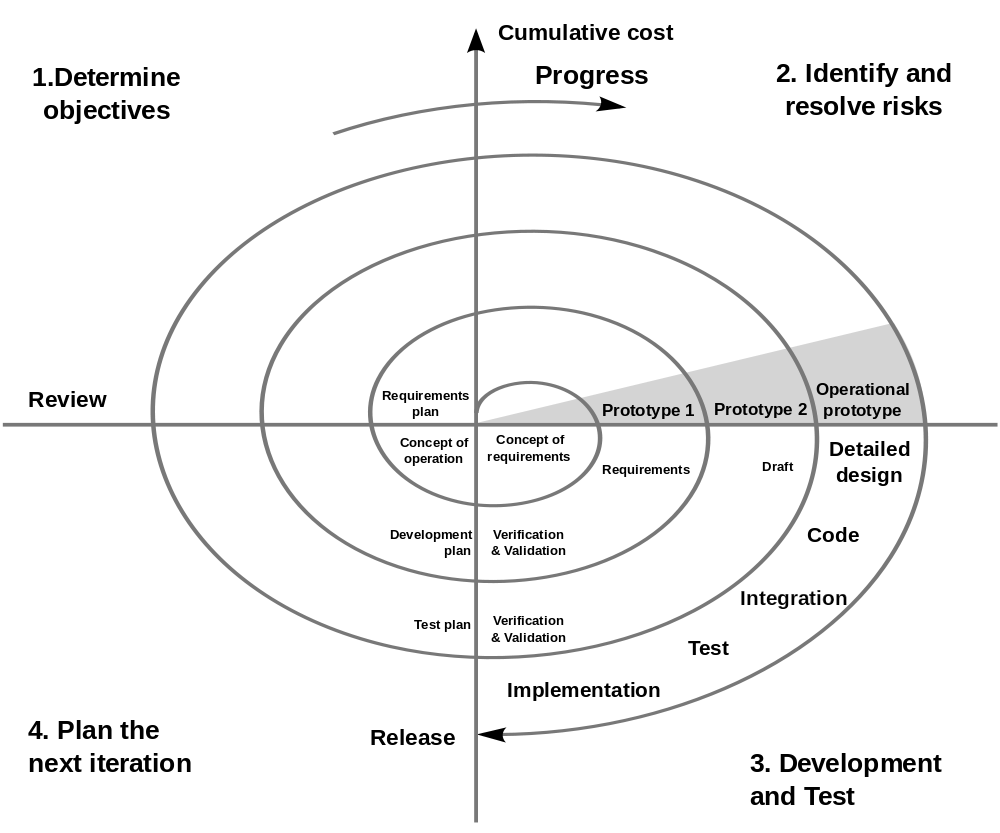
\includegraphics[width=0.6\textwidth]{imag/IMG17.png}
				\caption{Representación del desarrollo en espiral.} 
	\label{fig:Desarrollo en espiral.}	
	\end{center}
\end{figure}


\section{Plan de trabajo}
\hspace{1cm} Para conseguir la metodología de trabajo expuesta anteriormente se ha seguido una planificación dividida en las siguientes fases:

\begin{itemize}
	\item \textbf{Programación en Python:} Necesaria para poder entender el código anterior en el que me he basado y crear el mio propio. Con el conocimiento de c/c++ y una serie de guías de ayuda fue el  primer paso de aprendizaje.
	\item \textbf{Formación en JdeRobot:} Había que comprender el funcionamiento de la plataforma y saber todas las herramientas con las que contaba para saber en que te podías basar y que era lo que tenias que desarrollar tu mismo. Para ello se realizaron una serie de programas simples en los cuales trabajabas con distintos robots y con diferentes herramientas, teniendo así los primeros contactos con programación de robots simulados y reales.
	\item \textbf{Familiarización con Gazebo:} El simulador utilizado preferentemente en JdeRobot, en el hubo que crear el entorno de simulación sobre el cual se basaría el programa de vuelo del drone.	
	\item \textbf{Estudio y desarrollo del interfaz gráfico:} El programa se ha desarollado sobre la aplicación Visual States, la cual he tenido que aprender para conseguir introducir todas las etapas y que funcionase correctamente.
	\item \textbf{Aprendizaje e integración del componente de autolocalización:} Necesario para conocer el funcionamiento de este componente y poder manejar los parámetros y las balizas con las que trabaja, para así poder conseguir una correcta autolocalización del drone y tambien obtener los errores de la herramienta y extraerlos de los errores de pilotaje.
	\item \textbf{Adaptación y desarrollo del control de aterrizaje:} Para poder adaptarlo a la aplicación de Visual States y a su vez crear un propio sistema de despegue del drone.
	\item \textbf{Desarrollo del algoritmo para el control de pilotaje:} De dos formas diferentes, por un lado el algoritmo de seguimiento de puntos y por otro lado el de seguimiento de trayectorias. Ambos capaces de gobernar el movimiento del drone para seguir las rutas en 3D. 
	\item \textbf{Validación experimental en entornos simulados:} Para comprobar y validar el correcto funcionamiento de las fases anteriores se realizaron una serie de experimentos en entornos simulados, con estas pruebas se detectaron posibles comportamiento erróneos que corrigiéndolos se consiguió estabilidad en el sistema y una posible viabilidad en entornos reales.   
\end{itemize}

%\lhead[]{CAPÍTULO \thechapter. INFRAESTRUCTURA}
\chapter{Infraestructura}\label{cap.infraestructura}
\hspace{1cm} Una vez vistos los objetivos de este trabajo, en este capítulo se mostrarán las diferentes infraestructuras en las que nos hemos apoyado para la programación de la aplicación robótica de este TFG. También se explicara el funcionamiento de algunos componentes previos que hemos integrado.

\section{Gazebo}
\hspace{1cm} El simulador Gazebo es un programa open source distribuido bajo la licencia Apache 2.0 que se utiliza sobretodo para la investigación en robótica e Inteligencia Artificial.

\hspace{1cm} Este simulador ofrece la capacidad de simular de una forma eficiente y precisa cualquier tipo de robot en entornos complejos tanto de exterior como de interior. Sus características principales son sus motores de físicas, el motor de renderizado avanzado, el repositorio con la mayoría de robots comerciales y una gran gama de sensores y cámaras que permiten simular la mayoría de entornos reales.

\hspace{1cm} Al tratarse de un programa OpenSource su comunidad crece a diario lo que permite que cada ve existan más plugins, esto unido a la fácil integración en ROS e ICE permite que podamos tener el software base para simular los robots reales.
\\

\begin{figure}[H]
	\begin{center}
		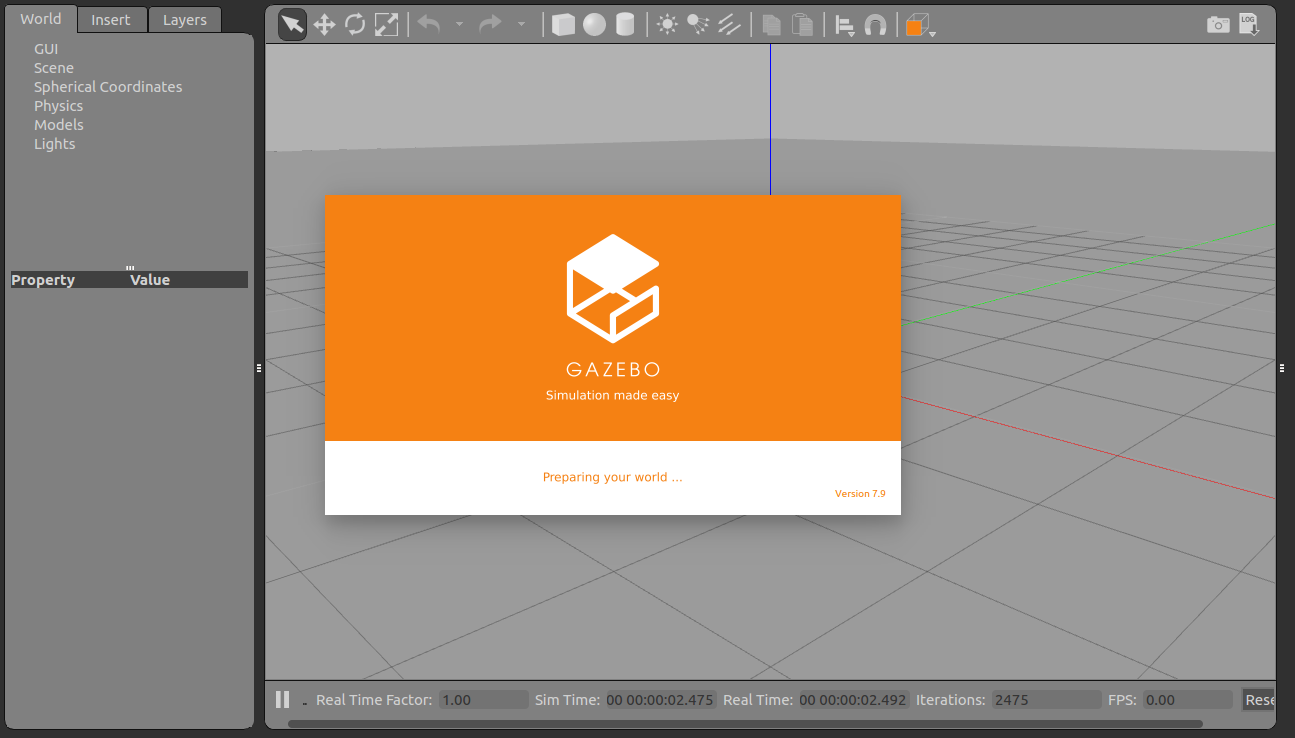
\includegraphics[width=1\textwidth]{imag/IMG18.png}
				\caption{Entorno de Simulación Gazebo.} 
	\label{fig:Gazebo.}	
	\end{center}
\end{figure}

\hspace{1cm} En nuestro TFG hemos trabajado con la versión Gazebo 7.9. Los mundos creados en esta aplicación se pueden lanzar sin GUI o con GUI y se definen con la extensión '.world' y escritos mediante SDF \textit{(Simulation Description Format)}.

\section{Balizas visuales AprilTags}
\hspace{1cm} AprilTags \cite{AprilTags2} es una biblioteca para el sistema de visión por computador que permite detectar balizas visuales contenidas en una imagen. Es útil en una amplia variedad de tareas que incluyen la realidad aumentada, la robótica y la calibración de cámaras.

\hspace{1cm} Las balizas se basan en el concepto de los códigos QR, aunque éstas están diseñadas para contener muchos menos bits de información(4-12 bits). Además, presenta un nuevo sistema de codificación que aborda problemas específicos de los códigos de barras 2D como es la robustez frente a la rotación y a los falsos positivos que pueden dar las imágenes naturales. EL software de detección AprilTag calcula la posición, orientación e identidad 3D precisa de las etiquetas en relación con la cámara, además de su correspondiente ID. Eso lo realiza mediante un algoritmo de segmentación basado en gradientes locales que consigue que las líneas se estimen con precisión, el cual se implementa en C sin dependencias externas. Esto provoca una tasa de falsos negativos muy bajos, aunque aumenta la probabilidad de falsos positivos. Sin embargo, gracias a la codificación de las balizas esta probabilidad es reducida hasta niveles aceptables.
\\

\begin{figure}[H]
	\begin{center}
		
\includegraphics[width=0.8\textwidth]{imag/IMG25.png}
				\caption{Ejemplos de AprilTags.} 
	\label{fig:AprilTags.}	
	\end{center}
\end{figure}

\hspace{1cm} Esta biblioteca la hemos utilizado como ayuda al sistema de autolocalización de Slam-VisualMarkers y su el código en C++ desarollado primero por Edwin Olson y posteriormente por Michael Kaess se puede obtener gratuitamente en su página \footnote{\url{http://people.csail.mit.edu/kaess/apriltags/}}, nosotros hemos utilizado su versión 2.1.

\section{Biblioteca OpenCV}
\hspace{1cm} OpenCV \footnote{\url{https://opencv.org/}} es una biblioteca \textit{open-source} de visión artificial que se desarrolló inicialmente por Intel, tiene un conjunto de funciones que van desde sistemas de seguridad con detección de movimiento hasta centros de procesamiento con reconocimiento de objetos. Está programada en C/C++ y en nuestro TFG para el procesamiento de imágenes nos hemos apoyado principalmente sobre ésta, trabajando en la versión 3.4. 

\hspace{1cm} Gracias a OpenCV, al obtener la imagen que transmite el drone se puede tanto detectar objetos como aplicar cambios sobre ella, para marcar las zonas de interés o diferentes objetos. Permite la realización de filtros de color, para eliminar objetos no deseados dependiendo el momento. Además permite el uso de operadores morfológicos (erosión y dilatación) gracias a los cuales se evitan imperfecciones en las imágenes como puede ser el ruido, que clasifica objetos inexistentes o de no interés como objetos de interés. En nuestro caso, nos ha servido tanto para la localización de las balizas de despegue y aterrizaje, como para la clasificación de las balizas AprilTag según la distancia a la que se encuentran del drone y por tanto el peso que tienen a la hora de calcular la posición.
\\

\begin{figure}[H]
	\begin{center}
		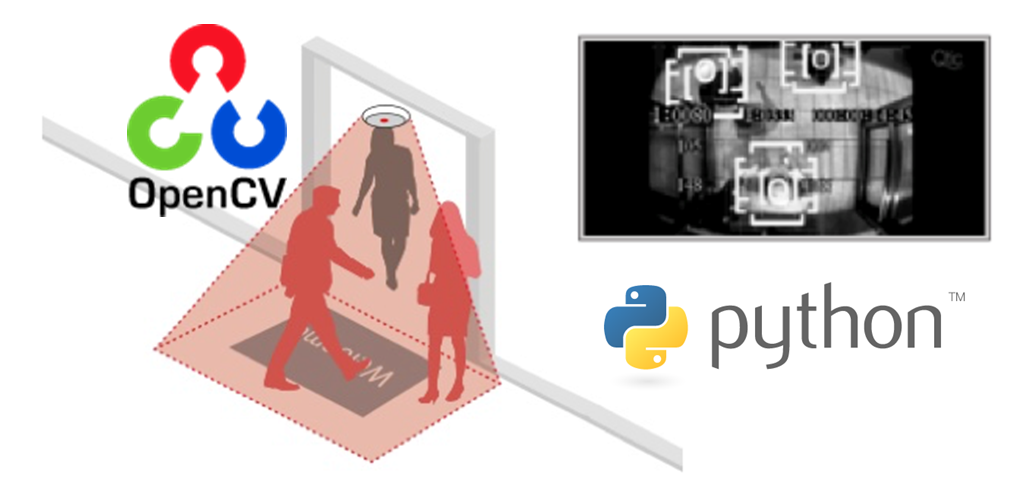
\includegraphics[width=0.8\textwidth]{imag/IMG26.png}
				\caption{Ejemplo de algoritmo con OpenCV.} 
	\label{fig:OpenCV.}	
	\end{center}
\end{figure}

\section{Biblioteca NumPy}
\hspace{1cm} Como hemos dicho este TFG está escrito en el lenguaje de programación Python y NumPy \footnote{\url{http://www.numpy.org/}} es una extensión \textit{open-source} de este lenguaje. Es el paquete fundamental para la informática científica con Python. Contiene, entre otras cosas un poderoso objeto de matriz N-dimensional, herramientas para integrar el código C/C++ y Fortran, álgebra lineal útil, transformadas de Fourier y capacidad de trabajo sobre números aleatorios. 

\hspace{1cm} Además de sus usos científicos obvios, NumPy también se puede usar como un contenedor multidimensional de datos genéricos. A su vez se pueden definir tipos de datos arbitrarios, lo que permite a NumPy integrarse de manera rápida y sin problemas con una amplia variedad de bases de datos. NumPy está licenciado bajo la licencia BSD \textit{(Berkeley Software Distribution)}, lo que permite su reutilización con pocas restricciones.

\section{Entorno JdeRobot}
\hspace{1cm} JdeRobot \footnote{\url{http://jderobot.org/Main_Page}} es un paquete de software libre para desarrollar aplicaciones de robótica y visión por computación. Estos dominios incluyen sensores como cámaras, actuadores y software inteligente en el medio. Está escrito principalmente en los lenguajes C++ y Python, y proporciona un entorno de programación basado en componentes. Pueden ejecutarse en diferentes ordenadores y se conectan mediante el middleware de comunicación ICE o los mensajes ROS. Los componentes interoperan a través de interfaces explícitas. Es el software principal con le que he trabajado y esta mantenido por el grupo de robótica de la Universidad Rey Juan Carlos.

\hspace{1cm} Para nuestro trabaja hemos utilizado la versión mas reciente del repositorio, JdeRobot-5.6.3(Febrero 2018) \footnote{\url{https://jderobot.org/Installation}}. Nos ha servido como herramienta para comprender los componentes previos que hemos utilizado del repositorio y la aplicación final es un conjunto de nodos desarrollados en el ecosistema JdeRobot.

\subsection{Herramienta ColorTuner}
\hspace{1cm} Es una aplicación para configurar filtros de color personalizados en espacios de color HSV, RGB o YUV, y así poder obtener la gama de color que nos interesa o realizar un filtro sobre una imagen o vídeo. Utiliza un interfaz ICE donde se representan dos imágenes, una la real y otra la filtrada, en esta se pueden variar los parámetros para ver que colores cumplen las características, quedándose los otros en negro. Se ha utilizado para extraer los colores de las balizas de aterrizaje y despegue y así poner su gama de colores correctamente en la aplicación final para que el drone las encuentre sin problemas.

\begin{figure}[H]
	\begin{center}
		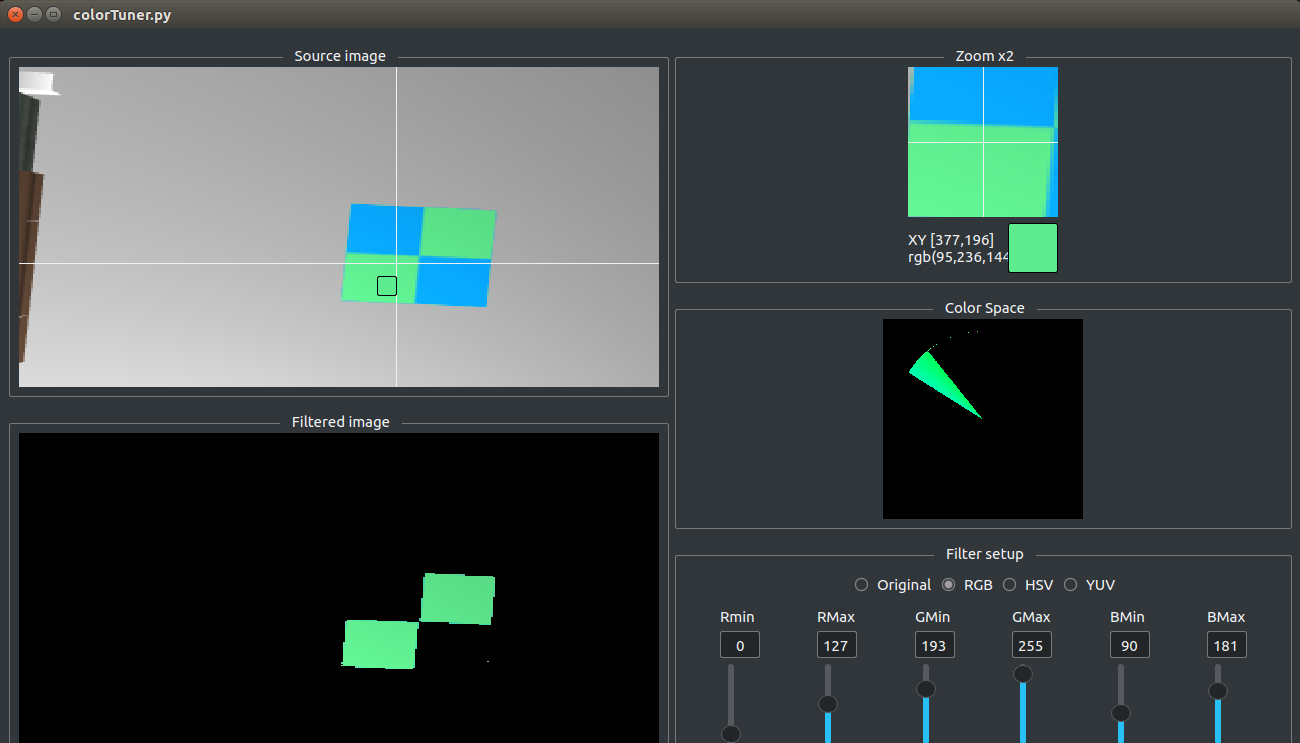
\includegraphics[width=1\textwidth]{imag/IMG27.png}
				\caption{Herramienta ColorTuner.} 
	\label{fig:ColorTuner.}	
	\end{center}
\end{figure}

\subsection{Plugin ArDrone2 en Gazebo}
\hspace{1cm} Hemos empleado para el desarrollo del proyecto el ArDrone 2.0 o más bien su modelo en el entorno de simulación Gazebo. Este plugin implementa un control realista y optimizado en simulación del drone, por lo que nos permite trabajar con los distintos sensores. Este drone cuenta cuenta con sensores IMU y con dos camaras una frontal y ora ventral, con ello y gracias al simulador Gazebo es capaz de ofrecer datos como pa posicion del drone o las imagenes que ve el mismo. También cuenta con una brújula, un altímetro y cuatro motores cada uno con su correspondiente hélice lo que nos permite enviar al drone una serie de comandos mediante el plugin \textit{CMDVel} para dirigir sus movimientos y saber en todo momento en que posición se encuentra.

\subsection{Interfaz Pose3D}
\hspace{1cm} Pose3D es la interfaz que se emplea en JdeRobot para obtener la posición y orientación en un espacio 3D de un objeto, en nuestro caso un drone. Se implementa mediante la función \emph{Pose3Ddata} y esta compuesta por un punto en 3D el cual indica la situación de un objeto mediante la posición en coordenadas cartesianas y la orientación mediante los cuaterniones, a partir de estos podremos obtener los ángulos de roll, pitch y yaw.

\begin{figure}[H]
 \centering
  \subfloat[Datos de Pose3DData]{
   \label{f:Pose3DData}
    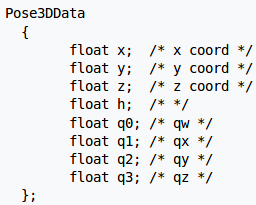
\includegraphics[width=0.25\textwidth]{imag/IMG20.png}}
  \subfloat[Representación de los datos]{
   \label{f:Datos}
    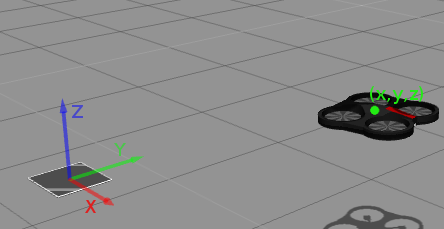
\includegraphics[width=0.35\textwidth]{imag/IMG21.png}} 
  \subfloat[Matriz de Conversión Angular]{
   \newline\label{f:Matriz Angular}
    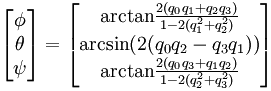
\includegraphics[width=0.35\textwidth]{imag/IMG22.png}} 
 \caption{Ejemplo de Pose3DData}
 \label{f:Ejemplo de Pose3DData}
\end{figure} 

\section{Visual States}
\hspace{1cm} VisualStates es una herramienta para la programación de comportamientos de robots que utilizan máquinas de estados finitos jerárquicas \textit{(HFSM - Hierarchichal Finite State Machine)} que permite el diseño gráfico de la inteligencia de un robot expresándola como estados y transiciones, además genera automáticamente un nodo JdeRobot en python que lo materializa. Representa el comportamiento del robot gráficamente en una hoja en blanco compuesto por estados y transiciones. Cuando el autómata está en un cierto estado, pasará a otro dependiendo de las condiciones establecidas en las transiciones. Esta representación gráfica permite un mayor nivel de abstracción para el usuario, ya que solo tiene que preocuparse por programar las acciones actuales del robot y seleccionar qué componentes puede necesitar de la interfaz del robot.

\hspace{1cm} Esta herramienta cuenta con una interfaz de usuario, la cual varia según estemos modificando el código o ejecutándolo. La GUI de visualStates permite el diseño de autómatas y la GUI de tiempo de ejecución de python proporciona una visualización del autómata en ejecución. 
\\

\begin{figure}[H]
	\begin{center}
		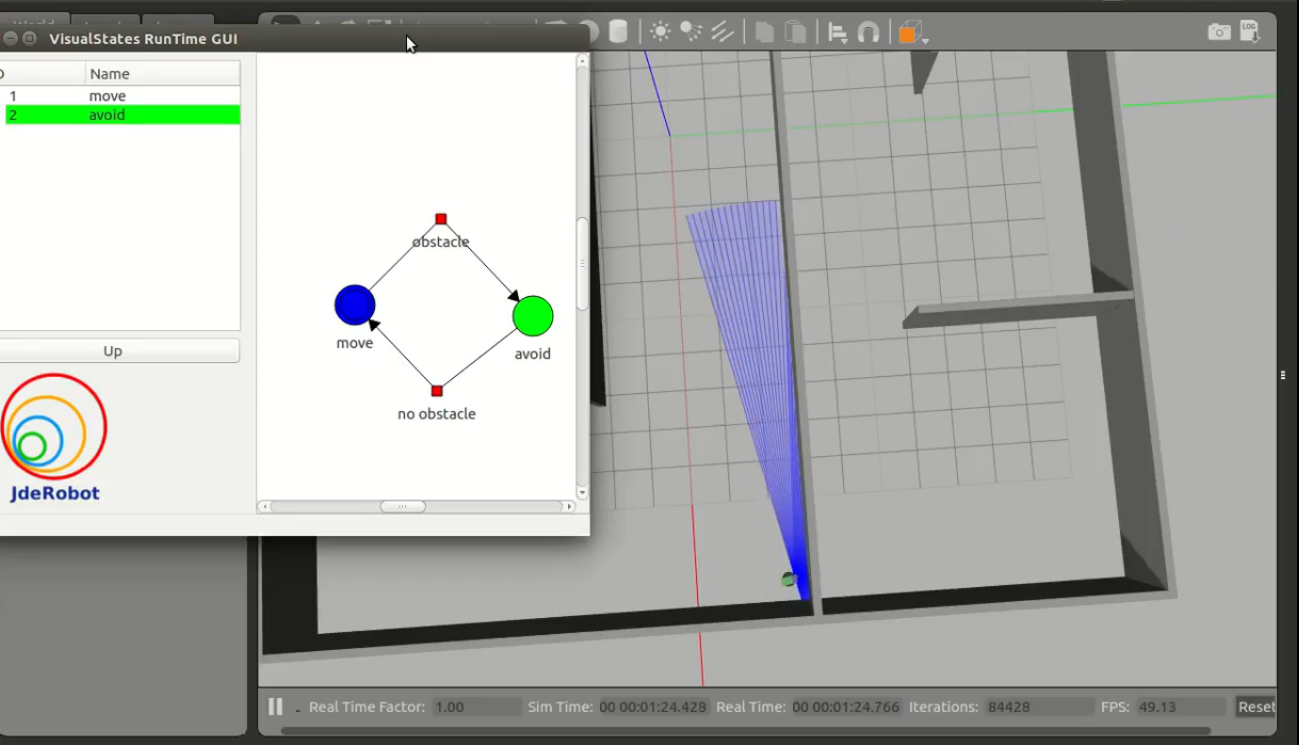
\includegraphics[width=1\textwidth]{imag/IMG19.png}
				\caption{Herramienta Visual States sobre Gazebo} 
	\label{fig:Visual States.}	
	\end{center}
\end{figure}

\hspace{1cm} En nuestro TFG hemos utilizado esta herramienta para la creación de nuestro propio autómata, gracias a ello hemos podido dividir el problema final en subapartados y así solucionarlos poco a apoco hasta llegar al algoritmo final. Se puede encontrar una guia de la herramienta en \footnote{\url{https://jderobot.org/Tutorials\#VisualStates_tool}}.

\section{Slam-Visualmakers}
\hspace{1cm} Es un nodo disponible en el ecosistema de JdeRobot que  mediante una serie de algoritmos capaces de localizar al sensor de forma simultánea a partir de balizas visuales proporciona la capacidad de autolocalización. Es una aplicación desarrollada por Felipe Pérez Molina \footnote{\url{http://jderobot.org/Flperezz-tfm}} en su Trabajo Fin de Máster que ha ido creando paralelamente a este TFG. Su trabajo esta desarrollado en la plataforma JdeRobot y está programada en C++. 

\begin{figure}[H]
	\begin{center}
		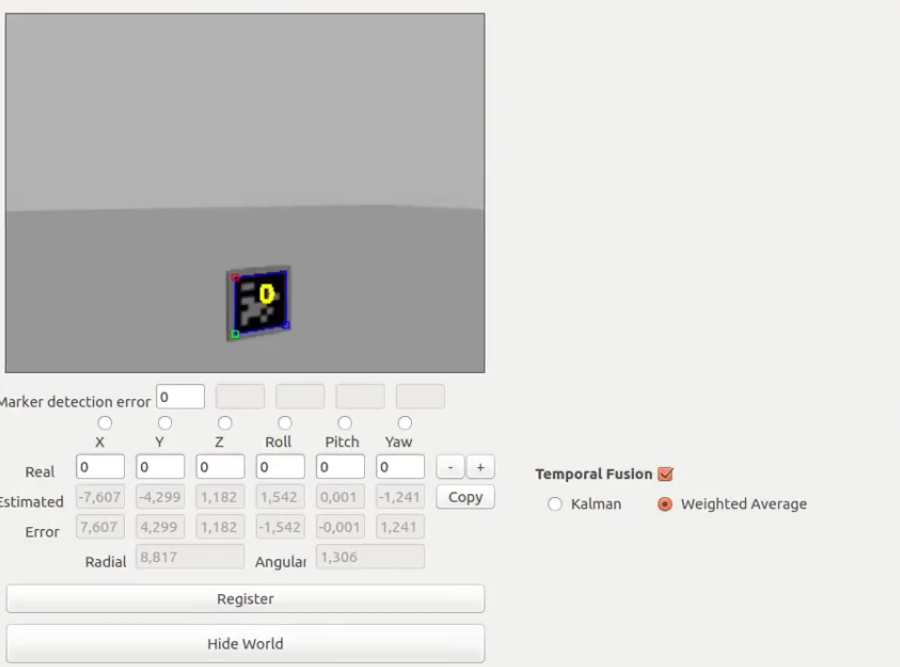
\includegraphics[width=0.6\textwidth]{imag/IMG24.png}
				\caption{GUI de Slam-Visualmarkers.} 
	\label{fig:GUI de Slam-Visualmarkers.}	
	\end{center}
\end{figure}

\hspace{1cm} Esta aplicación es un desarrollo de Cam-Autoloc, pero con un algoritmo de estimación de posición mas preciso, un interfaz gráfico propio, eliminando así la dependencia de QtCreator's, y la eliminación de la librería Aruco para su ejecución. 

\hspace{1cm} Para su correcto funcionamiento el algoritmo necesita tres entradas de datos: primero, se sirve de las imágenes recibidas a través de una interfaz creada con ICE y devuelve la posición estimada mediante un objeto Pose3D; segundo, un fichero de texto que contiene una lista donde figuran el identificador, posición y orientación 3D de cada baliza visual ubicada en el entorno; y tercero, otro fichero, este de configuración, que contiene toda la información de los parámetros de la cámara utilizada. 

\hspace{1cm} Para estimar la posición, el algoritmo comienza analizando la imagen recibida mediante las librerías OpenCV y AprilTags para explorar la imagen en 2D en busca de las balizas. Una vez localizadas, se hace uso de la librería Progeo para calcular la posición y orientación en tres dimensiones de la cámara con respecto a cada marcador. Finalmente, se realiza un proceso de fusión temporal y fusión espacial de las estimaciones obtenidas a partir de cada baliza. La aplicación permite elegir qué clase de filtro temporal utilizar, pudiendo escoger entre un filtro por pesos o un filtro Kalman.

\begin{figure}[H]
	\begin{center}
		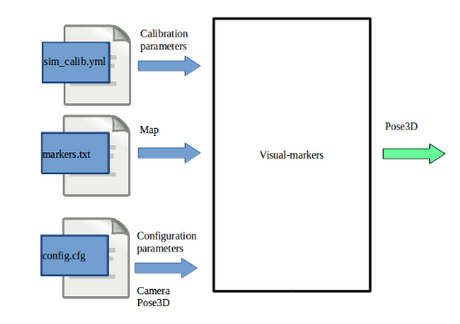
\includegraphics[width=0.6\textwidth]{imag/IMG23.png}
				\caption{Entradas y Salidas del nodo.} 
	\label{fig:Entradas y Salidas del nodo.}	
	\end{center}
\end{figure}

%\lhead[]{CAPÍTULO \thechapter. ALGORITMO}
\chapter{Navegación autónoma en seguimiento de rutas 3D}\label{cap.desarrollo}
\hspace{1cm} En este capítulo se describen los pasos seguidos para lograr una solución a los objetivos planteados, utilizando la infraestructura mencionada anteriormente y como se ha implementado.

\hspace{1cm} La solución al problema ha sido un algoritmo de navegación sobre el cual se dará una visión global. A continuación se explicará en detalle el diseño y el funcionamiento de cada uno de los componentes utilizados. Por último, se detallará cómo ha sido el proceso de integración y cual es la estructura del producto final.

%\hspace{1cm} Para explicar todo los pasos primero se dara un vistazo al diseño globalmente para posteriormente explicar cada uno de los modulos indicidualmete y así poder conocer todos ellos en detalle.

\section{Diseño}
\hspace{1cm} El objetivo de este algoritmo es que permitir al drone realizar un comportamiento completamente autónomo desde el despegue, hasta el aterrizaje, ambos controlados, pasando por el seguimiento de una ruta previamente definida. Todo esto basándose únicamente en balizas de apoyo visual. Por lo que estaríamos hablando del vuelo completamente autónomo de un drone mediante visión artificial y control de posición.

\hspace{1cm} En la aplicación final se diferencian dos partes principales: por un lado tenemos el componente encargado de estimar la posición mediante algoritmos de visión por computador y por otro lado tenemos el componente que se encarga del control del drone tomando las decisiones del movimiento según la etapa en la que se encuentre.

\hspace{1cm} En el esquema \ref{fig:Esquema representativo.} se puede ver una explicación de las entradas y salidas de flujos de información. También se pueden observar los ficheros que son imprescindibles en cada modulo para su correcto funcionamiento. Esta imagen nos da una idea del funcionamiento global de la aplicación y se puede observar como toda la comunicación entre procesos se lleva a cabo mediante ICE. A continuación vamos a explicar el comportamiento de cada módulo de una forma breve. 

\begin{figure}[H]
	\begin{center}
		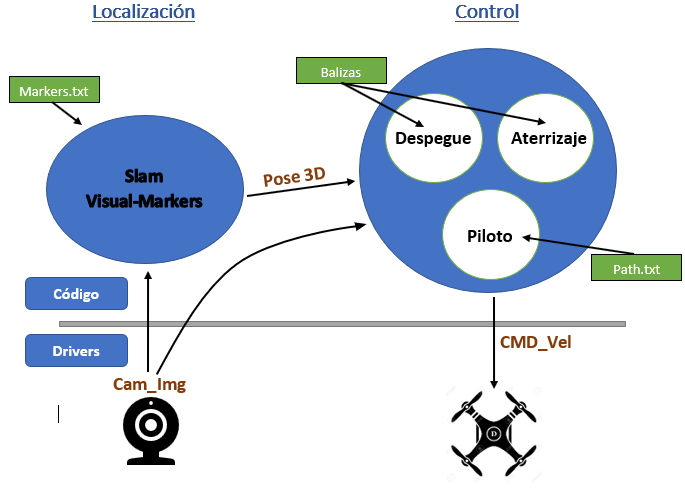
\includegraphics[width=1.1\textwidth]{imag/IMG31.PNG}
				\caption{Esquema representativo de la aplicación.}
		\label{fig:Esquema representativo.}	
	\end{center}
\end{figure}

\hspace{1cm} El módulo Slam VisualMarkers recibe las imágenes que le proporciona el drone y envia los datos en forma de Pose3D(x,y,z,q0,q1,q2,q3) a VisualStates. Este componente comienza analizando la imagen recibida en busca de la presencia de marcadores AprilTags. Si no los encuentra devuelve el número 0 como indicador de ello, en cambio si encuentra alguna envía cuántas ha encontrado y aplica cálculos de geometría proyectiva para estimar la posición de la cámara con respecto a cada una de las balizas. A continuación realiza una fusión espacial, aplicando un filtro basado en pesos y una fusión temporal, mediante un filtro de Kalman. Finalmente, la estimación calculada se envía al componente de navegación mediante una interfaz ICE.

\hspace{1cm} El módulo de Slam VisualMarkers recibe la imagen de la cámara del drone y las posiciones estimadas, envía estos datos a las etapas que lo necesiten y según en la etapa en la que se encuentre genera una serie de órdenes de velocidades que envía al drone vía interfaz ICE para conseguir el objetivo que según la etapa puede ser despegar, aterrizar o seguir una ruta.

\hspace{1cm} A continuación vamos a explicar cada modulo con mayor profundidad, nuestro mayor desarrollo en este TFG fue la creación de un algoritmo de pilotaje que mejorase los anteriores tanto en precisión de seguimiento de rutas como en tiempo de realización de estas rutas, por lo que sera el aparado en el que mas nos centraremos. Sin embargo, al ser un TFG de integración también explicaremos los módulos en los que nos hemos basado y hemos resintonizado para su correcto funcionamiento en el algoritmo final. 

\section{Componente de Autolocazalización} 
\hspace{1cm} Este modulo lo desarrollo originalmente Alberto López Cerón, luego fue refactorizado por Samuel Martín para integrar una capa de comunicaciones mediante interfaces ICE, también añadió métodos para la conversión entre cuaterniones y ángulos de Euler, debido a que la aplicación original utilizaba los ángulos de Euler y la interfaz Pose3D, cuaterniones, posteriormente Manuel Zafra la actualizo para jderobot e hizo los primeros pasos de navegación de drones utilizando esta autolocalización. Por último Felipe Pérez ha cambiado los ficheros de configuración para que sea una herramienta que funcione utilizando únicamente librerías que vienen en JdeRobot por si sola sin depender de QtCreator y su compilador \textit{qmake}, también esta creando la nueva infraestructura en ROS para que se pueda utilizar tanto en ICE como en esta, con la ventaja de que en ROS tendrá nuevos marcadores como el numero de balizas detectadas para poder hacer estudios de precision y marcas temporales para saber cuando entran las balizas en la aplicación y así caracterizar mejor el error de posición. 

\hspace{1cm} En cuanto a la herramienta Slam-VisualMarkers  está formada por un módulo principal \textit{Main-Window} que interconecta el resto de módulos e implementa una interfaz gráfica de usuario. El método \textit{ProcessImage} contenido en \textit{CameraManager} se ocupa de procesar la imagen en 2D capturada por la cámara y buscar en ésta la presencia de marcadores además de estimar la posición 3D con respecto a éstos. Es imprescindible el fichero de Markers.txt que contiene toda la información necesaria de cada marcador: id, tamaño y posición. Para localizar los marcadores en la imagen se hace uso del método de detección ofrecido por la biblioteca AprilTags. Este método se aplica a una versión en escala de grises de la imagen obtenida y tiene como salida un array en el que figuran todos los marcadores encontrados. Una vez el array de marcadores detectados es generado, se aplican una serie de operaciones geométricas. Estas operaciones devuelve la posición relativa de una cámara dado un sistema de referencia compuesto por la correspondencia entre los puntos 2D de la imagen y los correspondientes puntos 3D del mundo De esta forma se obtienen los vectores de translación y rotación del marcador con respecto a la cámara. Finalmente, la matriz que contiene la posición de la cámara con respecto al mundo se obtiene multiplicando la matriz calculada, posición del marcador con respecto a la cámara, y la matriz de posición del mundo con respecto al marcador. 

\begin{figure}[H]
	\begin{center}
		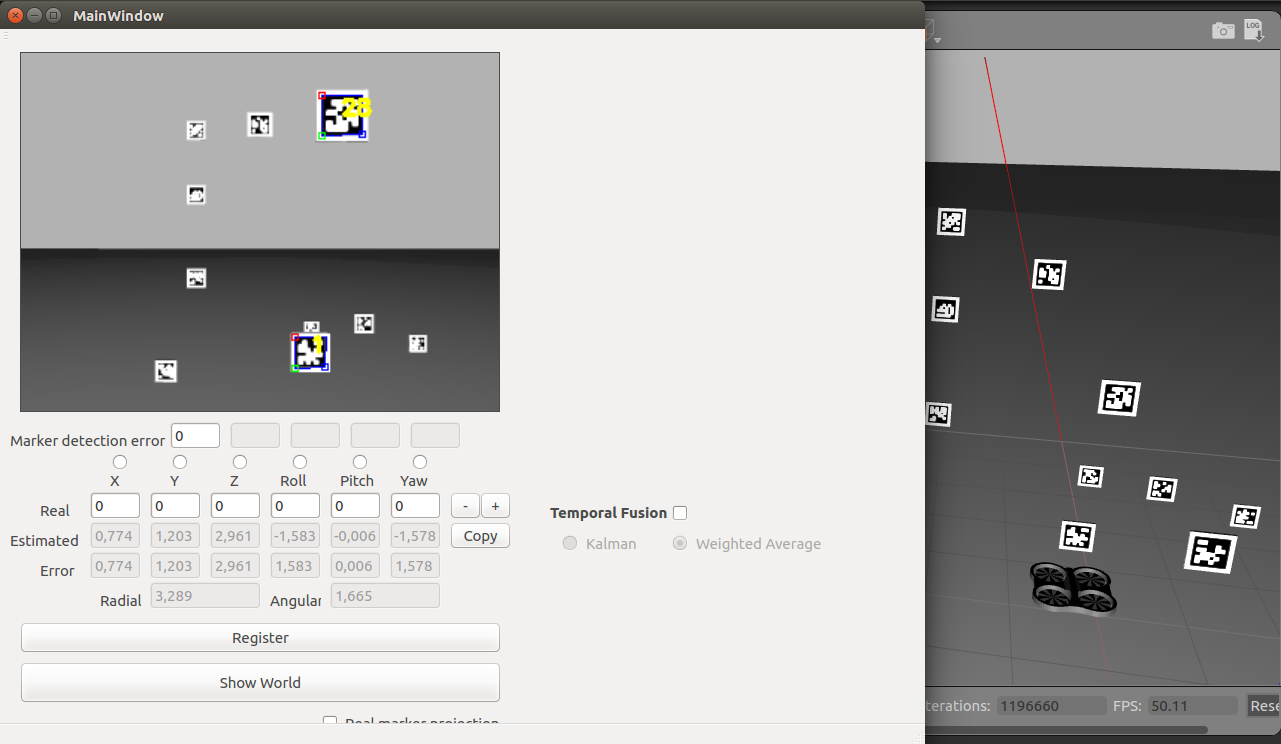
\includegraphics[width=0.85\textwidth]{imag/IMG35.png}
				\caption{Entorno de la aplicación Slam VisualMarkers}
		\label{fig:Ejemplo Slam VisualMarkers.}	
	\end{center}
\end{figure}

\hspace{1cm} Las posiciones estimadas para cada marcador son almacenadas en un array al que es aplicada una fusión espacial mediante un filtro por pesos. Este filtro asigna diferentes pesos a cada estimación basándose en la distancia a la cámara, de forma que los marcadores más cercanos son asignados con un peso mayor. En cuanto a los ángulos de rotación hay una operación especial, ya que no pueden ser sumados de la misma forma que las coordenadas lineales. Por último después de aplicar la fusión espacial, la aplicación original daba opción a aplicar una fusión temporal.  Esta fusión puede llevarse a cabo mediante un filtro por pesos como en el caso de la fusión espacial, o mediante la aplicación de un Filtro de Kalman \cite{FiltroKalman}.

\section{Componente de Control basado en estados}
\hspace{1cm} Todo el algoritmo de la aplicación se ha basado en un componente de control basado en estados, este componente se ha realizado con la herramienta de Visual States, la cual nos ha servido tanto para la creación del código como para la integración del sistema en un solo programa. 

\hspace{1cm} Visual Sates tiene la capacidad de crear estados, donde dentro se encuentra el código que se ejecuta, los cuales recorre mediante transiciones que pueden ser temporales o condicionales. Esto te permite centrarte en la escritura del algoritmo y de la conexión entre estados se encarga la aplicación. Además tiene otros módulos como las constantes y las funciones que una vez creadas se pueden utilizar en todos los estados y transiciones pudiendo así conectar y llevar un seguimiento de lo que ocurre en cada estado. Por último tenemos el apartado de las librerías, en el cual se introducen aquellas de las que depende tu programa, y el apartado de configuración, donde irán los diferentes enlaces a los interfaces de comunicación que hayamos utilizado. 

%\hspace{1cm} Es la parte en la que mas nos hemos centrado y que mas hemos conseguido desarrollar dentro del algoritmo, ya que para nosotros es la parte mas importante. Se podría decir que se trata de un piloto el cual realiza las tareas de pilotaje del drone. Hemos dividido el pilo según los datos que recibe de la interface de VisualStates.

\begin{figure}[H]
	\begin{center}
		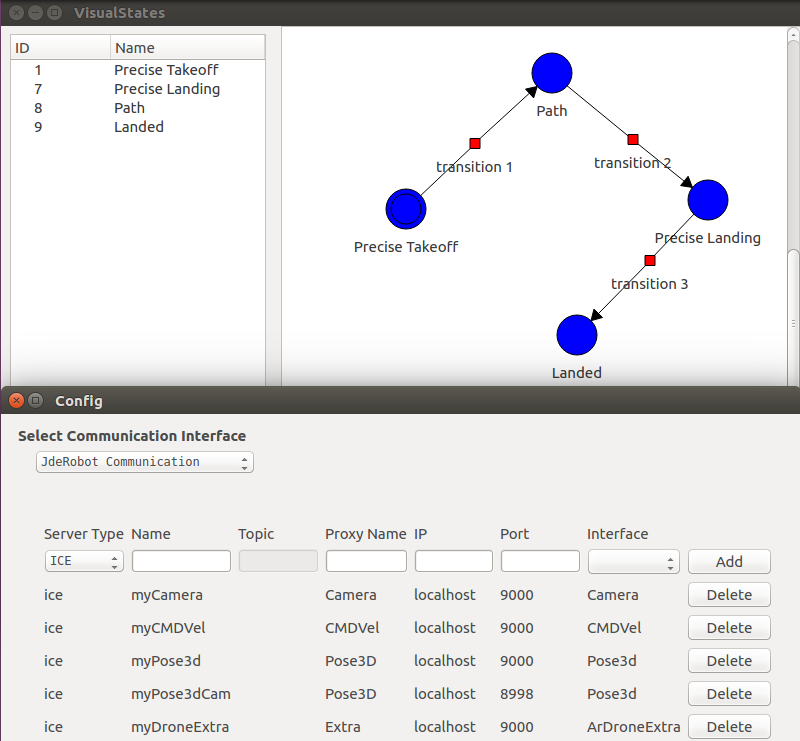
\includegraphics[width=0.8\textwidth]{imag/IMG32.png}
				\caption{Esquema de los componentes de Visual States.}
		\label{fig:Esquema VisualStates.}	
	\end{center}
\end{figure}

\section{Estados de despegue y aterrizaje}
\hspace{1cm} Para este componente hemos utilizado el trabajo que realizó Jorge Vela en su TFG \cite{JorgeVela} refactorizandolo y acoplándolo dentro de nuestro módulo de pilotaje en Visual States. El diseño de este algoritmo es un proceso basado en adquisición-procesado-envío de ordenes.  La adquisición de los datos se realizan mediante los sensores del drone. Estos datos sensoriales serán recogidos para su procesamiento y tras esto se enviarán las instrucciones al drone para que las ejecute. El sensor  utilizado en este estado ha sido la cámara, y a diferencia del estado anterior, los movimientos del drone dependerán de lo que esta capte en cada momento.

\hspace{1cm} El lugar de aterrizaje del drone es una baliza previamente definida \ref{fig:Baliza.}. Esta baliza es un cuadrado que en su interior tiene cuatro cuadrantes, dos verdes, y dos azules. Esta baliza se diseñó así para que sea difícil confundirla con otro objeto, pues de ser una baliza simple se podrían confundir los colores, además lo que busca el software será la cruceta que forman estos cuatro cuadrados y el punto central de ésta.

\begin{figure}[H]
	\begin{center}
		
\includegraphics[width=0.4\textwidth]{imag/IMG33.png}
				\caption{Baliza utilizada en Gazebo.}
		\label{fig:Baliza.}	
	\end{center}
\end{figure}

\hspace{1cm} En cuanto al \textbf{despegue} se sitúa el drone sobre una baliza sobre la cual tiene que estabilizarse. De esta forma, al despegar detecta esta y trata de centrarse, evitando así que se desvíe por factores externos y quedándose en la situación correcta y pasando al siguiente módulo que seria el del piloto. 

\hspace{1cm} Una vez el cuadricóptero termina la ruta establecida, este procede a la siguiente etapa que es el \textbf{aterrizaje}, el cual se divide en dos partes, primero la búsqueda de la baliza de aterrizaje y luego el centrado de la baliza y la aproximación a esta. 

\hspace{1cm} En cuanto a la búsqueda, sigue una navegación en espiral de forma que irá rastreando la zona ampliando su giro de forma continua, hasta que
detecte una baliza. Si no se detecta una baliza, continuará el algoritmo de búsqueda en el punto donde se había quedado, aumentando con la amplitud de las espirales a la que se había llegado. Cuando se detecte, dejara el movimiento en espiral y haciendo que coincida el centro de la baliza con el centro de la imagen de la cámara.  Para realizar el movimiento de centrarse en la baliza se ha utilizado un control PD (proporcional y derivativo).  

\hspace{1cm} por ultimo una vez coincide la cruceta de la baliza con el centro de la imagen, comienza a descender de forma constante a la vez que va centrando imagen por si el drone se desvía por algún factor externo. Cuando el área que detecta la baliza es prácticamente el área de la baliza, en ese momento el drone desciende  hasta  posarse en el suelo, entonces para los motores y el estado cambia a al estado final de \textit{"Landed"}.

\begin{figure}[H]
	\begin{center}
		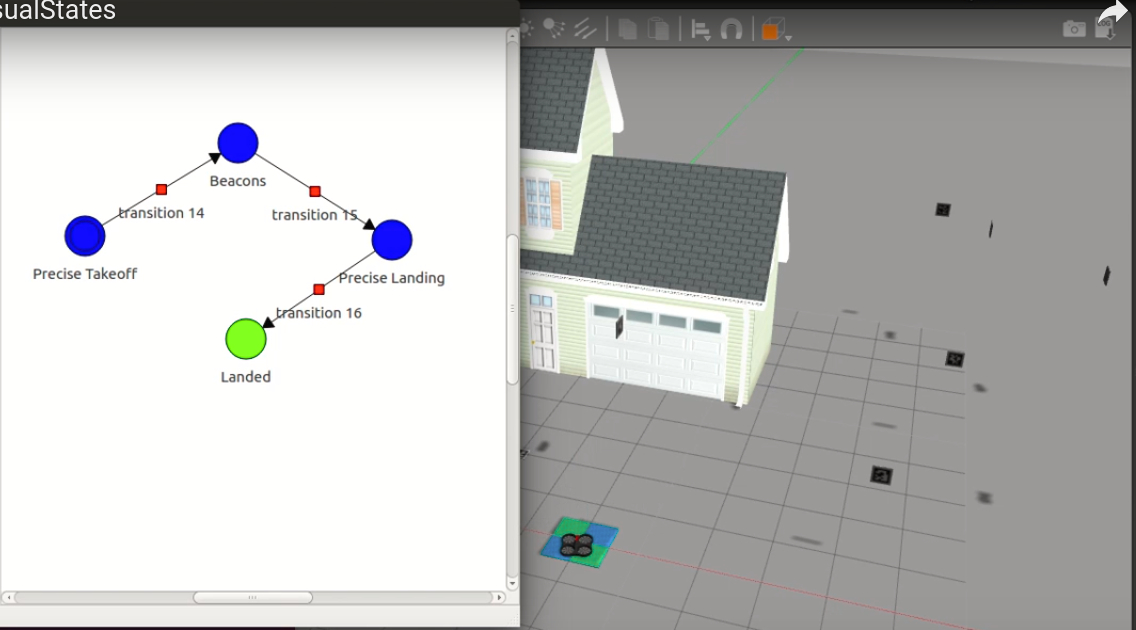
\includegraphics[width=0.9\textwidth]{imag/IMG34.png}
				\caption{Ejemplo de los estados en Visual States}
		\label{fig:Ejemplo Visual States.}	
	\end{center}
\end{figure}

\section{Estado de seguimiento de ruta}
\hspace{1cm} Como se puede observar en la imagen \ref{fig:Esquema VisualStates.} el algoritmo de este componente estaría en el estado de Path, el cual se encarga de seguir una trayectoria. Hemos desarrollado dos algoritmos diferentes según el tipo de trayectoria que se le introduzca, si es una trayectoria de puntos separados en la cual el drone solo tiene que alcanzar esos puntos se trataría del \textbf{Piloto por puntos de paso} si en cambio la trayectoria es una ruta de puntos prácticamente continuos y en la cual queremos que el drone mire hacia el siguiente punto al que se dirige entonces se trataría del \textbf{Piloto por trayectoria}. Ambos algoritmos se basan en la posición tridimensional del drone para ello hemos utilizado los tipos de datos de JdeRobot \textit{Pose3D} los cuales nos devuelven tanto la posición del drone como su orientación en el espacio mediante los cuaterniones o los Ángulos de Euler según lo que necesitemos. Estos datos serán proporcionados por la estimación de posición de Slam VisualMarkers. Y nuestro algoritmo devolvera una serie de velocidades que irá enviando al cuadricóptero mediante la función \textit{CMDVel()}.

\hspace{1cm} Por su sencillez de pilotaje vamos a explicar primero el \textbf{Piloto por puntos de paso}. Este control de pilotaje se centra en el movimiento direccional únicamente, es decir, para que el drone alcance el punto al que debe llegar no variara prácticamente ninguno de sus ángulos de Euler, tan solo se moverá sobre los ejes x,y,z.

\hspace{1cm} Como el movimiento sera únicamente direccional en coordenadas cartesianas tan solo hay que calcular el vector que apunta desde la posición del cuadricóptero hasta el siguiente punto de ruta que se desea alcanzar: 

\[Pose3D = (P_{x}, P_{y}, P_{z})\hspace{1cm};\hspace{1cm}Beacon = (B_{x}, B_{y}, B_{z})\]
\[\overrightarrow{V}_{x} = P_{x} - B_{x}\hspace{0.5cm};\hspace{0.5cm}\overrightarrow{V}_{y} = P_{y} - B_{y}\hspace{0.5cm};\hspace{0.5cm}\overrightarrow{V}_{z} = P_{z} - B_{z}\]

\hspace{1cm} Una vez calculado este vector entre las posiciones lo multiplicaremos por un coeficiente regulador que reducirá los valores hasta que estos se encuentren dentro del rango de velocidades del drone y una vez alcanzado este rango se pasaran los valores por una función que compruebe que las velocidades máximas no exceden las permisibles por Slam VisuaMarkers para la detección y análisis de balizas: 

\begin{lstlisting}[backgroundcolor=\color{gray!15}]
    if math.fabs(xVel) > MaxVx :
        xVel = MaxVx * np.sign(xVel)
    if math.fabs(yVel) > MaxVy :
        yVel = MaxVx * np.sign(yVel)
    if math.fabs(zVel) > MaxVz :
        zVel = MaxVx * np.sign(zVel)        
\end{lstlisting}

\hspace{1cm} Con este método de control de navegación por posición nos aseguraremos que el drone alcanza el punto que queremos adecuadamente y a medida que se va acercando a el, para que la aproximación sea exacta, al reducirse el vector se reducirá la velocidad alcanzando la baliza con total exactitud. Una vez se alcanza la baliza se busca cual es la siguiente en la lista y se vuelve a realizar el proceso, así hasta alcanzar todas ellas.

\hspace{1cm} En cuanto al \textbf{Piloto por trayectoria} lo primero fue crear las rutas que posteriormente seguiría el drone, como estas debían ser largas con giros y con puntos muy consecutivos se creo en python la función que nos permitiese crear estas según la separación entre puntos de ruta que considerásemos necesaria: 
\begin{lstlisting}[backgroundcolor=\color{gray!15}]
i=0
a=0
if i == 0:
    archivo = open('pos.txt','w')
    archivo.write('  x     y     z    roll   pitch   yaw \n')
    i = i+1
b = time.clock()
pos_sim = self.pose.getPose3d()
    if ((b - a) > time_write):
        archivo.write(str(pos_sim.x)+' ')
        archivo.write(str(pos_sim.y)+' ')
        archivo.write(str(pos_sim.z)+' ')
        archivo.write(str(pos_sim.roll)+' ')
        archivo.write(str(pos_sim.pitch)+' ')
        archivo.write(str(pos_sim.yaw)+' ')
        archivo.write(str(b)+'\n')
        a = b 
\end{lstlisting}

\hspace{1cm} Una vez obtenida la ruta y a diferencia del \textbf{Piloto por puntos de paso} este seguirá los puntos orientándose siempre en la dirección entre la posición y el siguiente punto, para ello tendremos que variar la velocidad angular en torno al eje Z, modificando por tanto el ángulo de yaw del drone y de esta forma conseguir orientarlo de la forma mas rápida hasta el siguiente punto de la ruta. Las primeras versiones del piloto tan solo se iban a tener en cuenta las velocidades lineales correspondientes a los ejes X y Z del drone, descartando la velocidad en Y debido a que modificando yaw no sería necesario el movimiento lateral. Pero con forme se fue investigando  mejorando esta versión se descubrió que permitir al drone realizar pequeñas variaciones en la velocidad lineal del eje Y permitía un aproximación a los puntos mucho mas efectiva y precisa, por lo que se optó por incluir también la variación de la velocidad en el eje Y. Con la ayuda del piloto anterior y teniendo en cuenta las mejoras anteriores se va a explicar el algoritmo final de pilotaje. 

\hspace{1cm} Para el cálculo de las velocidades lineales se seguirán los mismos pasos que en el \textbf{Piloto por puntos de paso} pero variaremos los coeficientes de corrección para que las velocidades lineales sean parejas a la nueva velocidad angular. Esta velocidad angular se calculara mediante las funciones de predicción de posición. 

\hspace{1cm} Para ello el primer paso es calcular la distancia horizontal que recorrerá el drone hasta la siguiente iteración del algoritmo. La distancia se obtiene multiplicando la velocidad horizontal obtenida anteriormente por el tiempo que transcurre entre dos iteraciones: \(d_{\psi} = v_{x} * \Delta_{t}\).

\hspace{1cm} Para predecir la posición del cuadricótpero debemos tener en cuenta el ángulo de giro con respecto al eje Z del drone en ese instante. Ya que en el estándar de Pose3D la orientación se indica en cuaterniones, haremos un conversión para conocer el ángulo de Euler mediante la siguiente ecuación:

\[ \Psi_{z} = arctan^{2}\left( \frac{2*q_{0}*q_{3}+q_{1}*q_{2}}{1-2*(q_{2}^{2}+q_{3}^{2})}\right) \]
 
\hspace{1cm} Una vez obtenido el ángulo $\Psi_{z}$ sacamos la posición que predecimos solo en X e Y ya que la variación en Z no influye en cálculo del ángulo de giro de yaw.

\[ X_{f} = d_{\psi} * cos \Psi_{z} + x_{pose} \] 
\[ Y_{f} = d_{\psi} * sin \Psi_{z} + y_{pose} \]

\hspace{1cm} Ahora calcularemos el error de ángulo, que es la diferencia entre el ángulo actual y el ángulo sobre el eje Z existente entre el drone y el punto de ruta, $\Psi_{e}$ Teniendo el ángulo se calcula una velocidad angular a partir de la distancia horizontal al punto, $d_{H}$, y la velocidad lineal actual, $v_{x}$.
 
\[\Psi_{path} = arctan \left(\frac{V_{y}}{V_{x}}\right)  \hspace{0.5cm};\hspace{0.5cm}\Psi_{e} = \Psi_{path} - \Psi_{z} \]

\[d_{H} = \sqrt{V_{x}^{2} + V_{y}^{2}} \hspace{0.5cm};\hspace{0.5cm} \omega_{e} =  \dfrac{\Psi_{e}}{d_{H}/v_{x}}\]

\hspace{1cm} La velocidad angular dependerá entonces de la velocidad angular calculada y de un factor de corrección que viene dado por la relación entre el error lateral predicho $L_{fe}$ y la velocidad horizontal. Este factor está multiplicado por una constante $K_{g}$, que es la ganancia de corrección del giro.

\[ L_{fe} = cos\Psi_{z}*(Y_{path}-Y_{f}) - sin\Psi_{z}*(X_{path}-X_{f}) \]
\[ \omega_{z} = \omega_{e} + K_{g} * (L_{fe}/v_{x})\]

\hspace{1cm} Por último, una vez obtenida la velocidad angular $\omega_{z}$ ajustaremos la velocidad en el eje Y, $v_{y}$, a partir de esta. Una vez obtenidas las tres velocidades que se van a enviar al drone, las velocidades horizontales $v_{x}$ $v_{y}$, la velocidad vertical $v_{z}$ y velocidad angular $\omega_{z}$ se envían al drone mediante una llamada al método \textit{SendCMDVel(vx,vy,vz,wz)}
de Interfaces, que se ocupa de mandar las órdenes decididas al cuadricóptero.

%\lhead[]{CAPÍTULO \thechapter. EXPERIMENTOS}
\chapter{Experimentos}\label{cap.experimentos}
\hspace{1cm} En este capítulo se describen los experimentos realizados para validar el prototipo final, para comprobar el correcto funcionamiento del algoritmo completo y llegar a una solución final tras depurar mientras se desarrollaba. Para ello se ha dividido el capítulo en cuatro partes a analizar: la primera parte, se ha comprobado la calidad de autolocalización, es decir, se ha realizado una ruta teleoperada para ver los errores de posición de la aplicación; en la segunda se ha validado el
nuevo módulo de despegue; la tercera parte, se ha evaluado la calidad del controlador, es decir, el error que comente el piloto al realizar una ruta predefinida. Y por último, se ha validado el funcionamiento de la aplicación final con todos los componentes a la vez.

\hspace{1cm} Dada la complejidad de los experimentos, se han llevado a cabo dentro del entorno de simulación Gazebo. El plugin para la simulación del comportamiento del dron, así como el modelo necesario para la renderización del vehículo y sus sensores están incluidos en JdeRobot. Pero para realizar correctamente los diferentes experimentos se han creado una serie de mundos en 3D, los cuales cuentan con espacios abiertos, espacios cerrados, balizas arlequinadas y balizas AprilTags con sus correspondientes texturas. Los mundos creados se han integrado en el repositorio oficial de JdeRobot bajo los nombres de \textit{ArDrone1}, \textit{ArDrone2} y \textit{ArDrone3}.

\hspace{1cm} En la Figura \ref{fig:Mundo Gazebo.} se puede observar el mundo ArDrone1, que fue el primero que creamos y el más representativo ya que se puede observar una posible aplicación de reconocimiento de un casa mediante el dron completamente automatizado. Cuenta con las balizas arlequinadas de despegue (verde-naranja) y aterrizaje (verda-azul), con balizas 23 AprilTags para la autolocalización que rodean una casa a la cual el dron tiene que darle una vuelta completa.

\begin{figure}[H]
	\begin{center}
		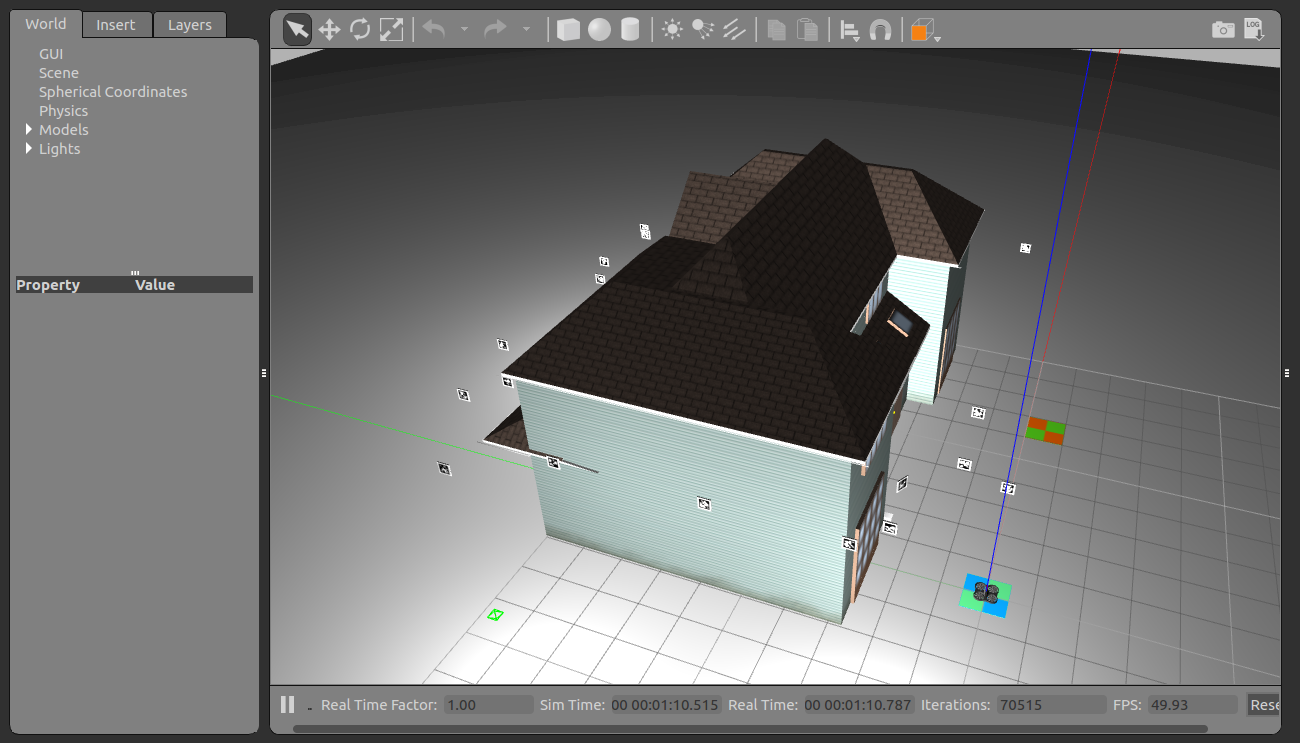
\includegraphics[width=1\textwidth]{imag/IMG28.png}
				\caption{Mundo Gazebo ArDones1.}
		\label{fig:Mundo Gazebo.}	
	\end{center}
\end{figure}

\hspace{1cm} Tanto para el cálculo de trayectorias, como para el cálculo de errores de distancia y de tiempos de ruta, se ha hecho uso del programa Matlab, el cual nos ha facilitado todos los procesos de cálculo.

\section{Pruebas unitarias de autolocalización}
\hspace{1cm} Para evaluar el comportamiento del componente \texttt{Slam VisualMarkers} que se encarga de la autolocalización del dron, se aisló completamente de la parte de pilotaje. Para ello lo que se hizo fue teledirigir a mano el dron dentro de un mundo de balizas el cual permitiese al componente ver al menos una baliza AprilTag en todo momento de la ruta. Una vez terminada la ruta se comparó la secuencia de posiciones reales entregada por el simulador $P_{0}$ con la secuencia de posiciones estimadas por el componente $P_{A} $. Dado que ambas entregan tanto posición (x y z) como dirección (Pitch Roll Yaw) se realizó un cálculo de error de posición mediante la distancia euclídea: 
\[ E_{p} = \sqrt{(P_{Ax}-P_{0x})^{2}+(P_{Ay}-P_{0y})^{2}+(P_{Az}-P_{0z})^{2}}\]
y lo que hemos definido como el \textit{error angular}:    
\[ E_{a} = \sqrt{(P_{AP}-P_{0P})^{2}+(P_{AR}-P_{0R})^{2}+(P_{AY}-P_{0Y})^{2}}\]

\begin{figure}[H]
	\begin{center}
		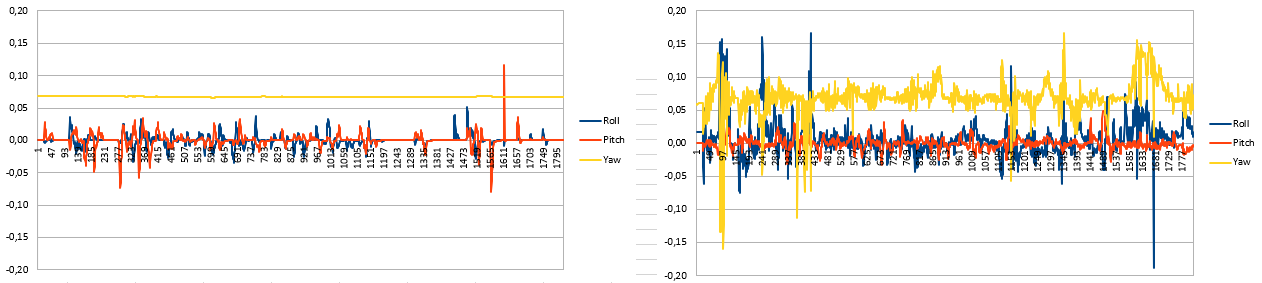
\includegraphics[width=1\textwidth]{imag/IMG90.PNG}
				\caption{Diferencia angular entre lo real y VisualMarkers}
		\label{fig:Error angular.}	
	\end{center}
\end{figure}

\begin{figure}[H]
	\begin{center}
		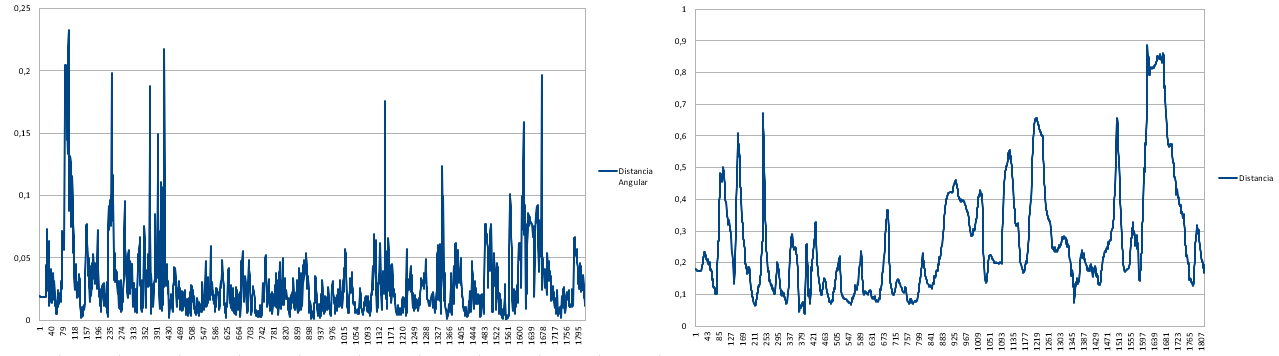
\includegraphics[width=1\textwidth]{imag/IMG91.PNG}
				\caption{Cálculo de errores de distancia y de ángulos}
		\label{fig:Error de distancia y de giro.}	
	\end{center}
\end{figure}

\hspace{1cm} Con la aplicación de las fórmulas anteriores se obtuvieron las gráficas de la figura \ref{fig:Error de distancia y de giro.}. En las gráficas superiores se ve la diferencia entre los tres ángulos pitch, roll y yaw del dron real (izquierda) con los calculados por el componente Slam VisualMarkers (derecha). Comparando visualmente las gráficas parece que el error sea elevado pero una vez analizados numéricamente los datos y calculando los errores con la fórmula anterior y representándolos en la gráfica izquierda de la Fig \ref{fig:Error de distancia y de giro.} se ve como el error angular medio es de 0.0293rad lo que equivale a 1.679 grados, que es un error muy pequeño, el error angular máximo es de 0.2329rad que son 13.344 grados. Por último. la gráfica derecha de la Fig \ref{fig:Error de distancia y de giro.} nos muestra los errores de distancia euclídea entre la ruta realizada realmente con la posición que se calculaba con Slam-VisualMarkers, esta nos da que el error medio de distancia euclídea es de 0.2651m y el error máximo de distancia euclídea es de 0.8856m. Con el cálculo de estos números y teniendo en cuenta que los errores máximos se producen cuando el dron sólo ve una baliza y esta está alejada son cifras bastante razonables.

\begin{figure}[H]
	\begin{center}
		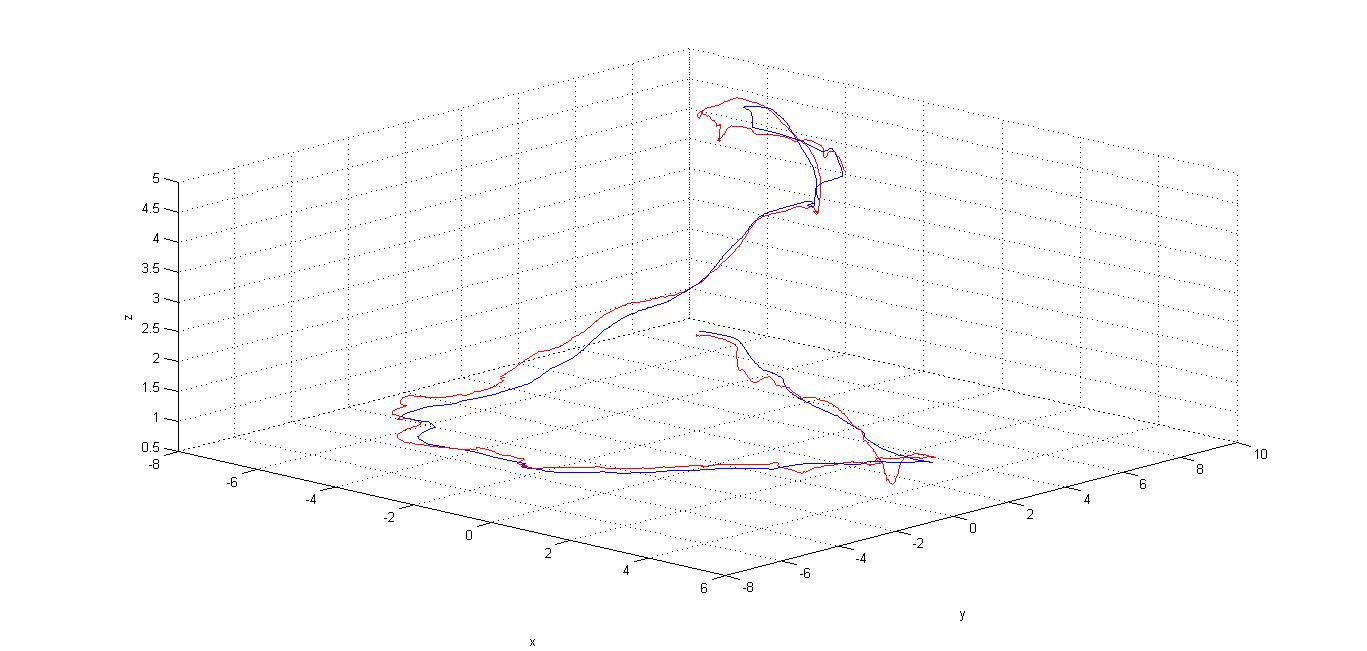
\includegraphics[width=1\textwidth]{imag/IMG48.jpg}
				\caption{Cálculo de posición de Slam-VisualMarkers}
		\label{fig:Comparativa Slam-Visualmarkers.}	
	\end{center}
\end{figure}

\hspace{1cm} Una vez realizados los cálculos del error se comprobó como cuando el componente pierde de vista las AprilTags los errores de posicionamiento aumentan considerablemente como se puede observar en la Figura \ref{fig:Comparativa Slam-Visualmarkers.}, en la cual tenemos la ruta realizada en azul y la ruta estimada por el componente en rojo. Para evitar esto se habló con el desarrollador de Slam VisualMarkers y se añadió más información a su interfaz de salida en ROS de modo que ya indicaba el número de balizas que se estaban viendo.

\hspace{1cm} Esta caracterización experimental de la autolocalización permitió acotar los márgenes de error con los que tenía que lidiar el nodo de pilotaje y permitió mejorar la navegación autónoma contemplando la situación en la que el dron se perdía. Con esto se pudo crear un nuevo comportamiento que permite que cuando el dron no esté viendo ninguna baliza no siga la ruta, sino que gire sobre sí mismo realizando círculos, cada vez mayores, sobre el último punto donde veía alguna baliza, para así poder volver a encontrarla y posicionarse correctamente. Esto ayudó a que el dron no se perdiese de la ruta y siguiese moviéndose cuando no encontraba ninguna baliza, ya que ahora si da tres vueltas y seguía sin encontrar ninguna baliza, el dron aterriza. Con esta nueva función mejoramos la integridad de la aplicación de navegación autónoma y nos aseguramos de que el cuadricóptero no se aleje excesivamente de la ruta definida, preparándolo para los experimentos reales.

\section{Pruebas unitarias de despegue controlado}
\hspace{1cm} Ya que refactorizamos completamente el código de Jorge Vela para crear el despegue controlado a partir de su aterrizaje controlado, tuvimos que hacer una serie de experimentos hasta conseguir una version refinada satisfactoria. Una vez el dron se encuentra sobre una baliza arlequinada, éste es el primer estado de la aplicación. Este estado consta de cuatro partes que se pueden observar en la Figura \ref{f:Despegue controlado}: la primera parte es la puesta en marcha de los motores y al ascenso del dron hasta un altura que viene establecida por el propio dron, normalmente entre 0.5-1m, una vez el dron se ha puesto en marcha, entramos en el segundo apartado en el cual el dron centra la cruceta de la baliza arlequinada con el centro de la cámara. A continuación llega el tercer apartado en el cual realiza un ascenso controlado, esto es, va subiendo a una velocidad constante hasta que detecta que la cruceta de la baliza no está centrada con la cámara, se vuelve a cuadrar y sigue ascendiendo. Así hasta que entramos en el cuarto paso en el cual la baliza se ve, en la imagen que proporciona el dron, como una quinta parte del total, una vez llegado a este punto cesa el ascenso y se mantiene a esta distancia pasando al siguiente estado del algoritmo, el seguimiento de una ruta. 

\begin{figure}[H]
 \centering
    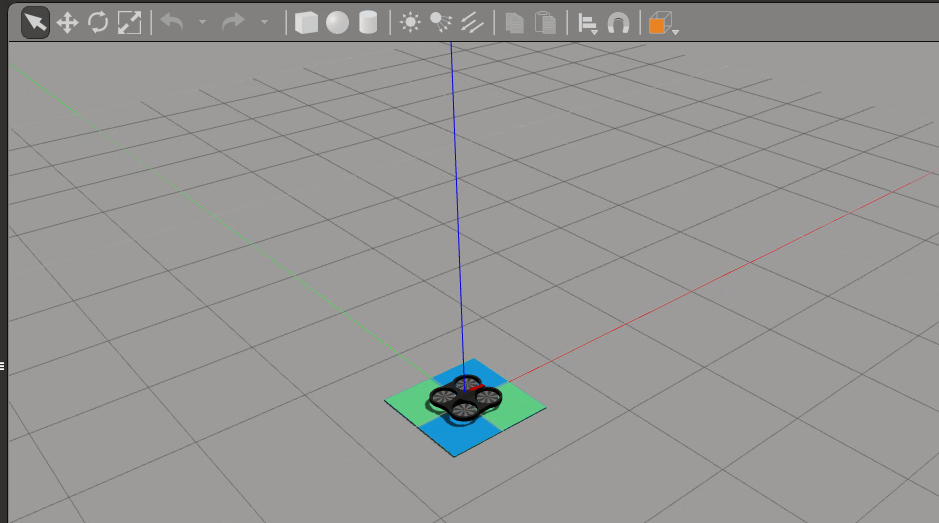
\includegraphics[width=7.6cm,height=4cm]{imag/IMG99.png}
    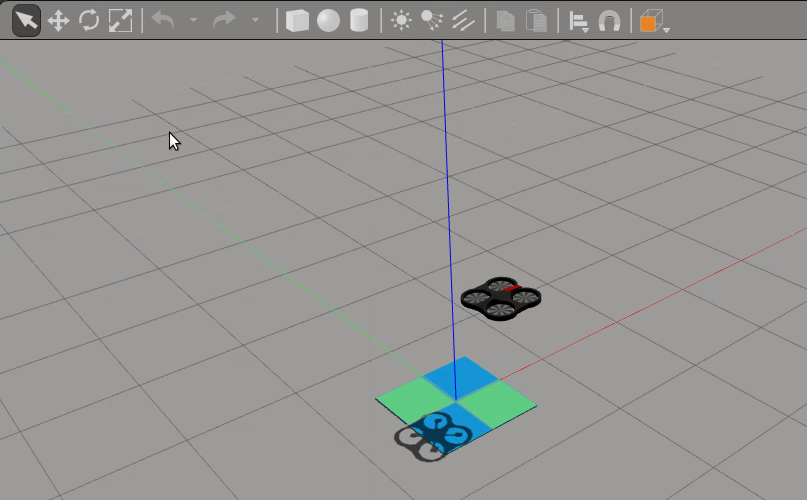
\includegraphics[width=7.6cm,height=4cm]{imag/IMG98.png}
    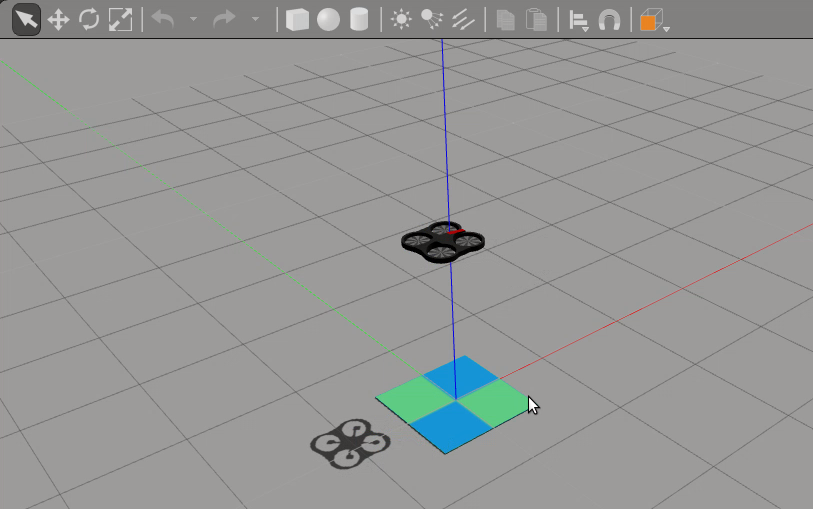
\includegraphics[width=7.6cm,height=4cm]{imag/IMG97.png}
    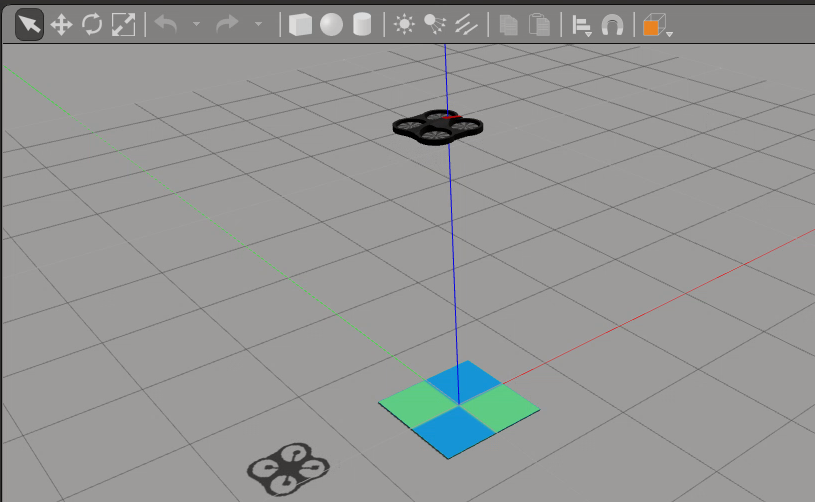
\includegraphics[width=7.6cm,height=4cm]{imag/IMG96.png}
 \caption{Pasos en el despegue controlado}
 \label{f:Despegue controlado}
\end{figure}

\section{Pruebas unitarias de pilotaje}
\hspace{1cm} A diferencia de las pruebas anteriores, en estas pruebas se suministraba al piloto la posición verdadera del dron en todo momento, extraida del simulador. Así, los errores entre la ruta deseada y la realmente conseguida son exclusivamente achacables al pilotaje, no a la autolocalización. 

\subsection{Pilotaje por puntos de paso}
\hspace{1cm} El primer piloto desarrollado se encargaba de seguir únicamente puntos de paso, es decir tan solo variaría la velocidad lineal del dron. Los primeros experimentos mostraban como el piloto se acercaba correctamente al punto, pero en la aproximación final no lograba alcanzarlo, por lo que se tuvieron que realizar varias correcciones, tanto de velocidades máximas en los ejes x e y, como de variaciones de velocidad según la cercanía al siguiente punto de paso. Una vez conseguido esto se volvieron a ajustar los parámetros de velocidades máximas, esta vez en los tres ejes para conseguir que el error en una ruta por puntos nunca superase los 10cm. Para ello se tuvo que sacrificar la velocidad máxima cuando el dron se acercaba al siguiente punto de paso, pero aun así, la velocidad media del dron continuaba siendo el 0.82 de la máxima.

\hspace{1cm} En la Figura \ref{fig:Error asociado al pilotaje.} se puede ver una ruta por puntos compleja (en verde) y cómo ajustando la velocidad cercana a los puntos, la ruta final del dron es más exacta (rojo) que permitiéndole una velocidad máxima mayor (azul). Con todos estos ajustes y alternativas probadas, al final se ofrece un piloto que se puede configurar para que realice la ruta con mayor rapidez o con una mayor exactitud, recalcando que el error introducido por el pilotaje es aceptable, que consigue pasar por todos los puntos de paso especificados con un error por debajo de 1cm.

\begin{figure}[H]
	\begin{center}
		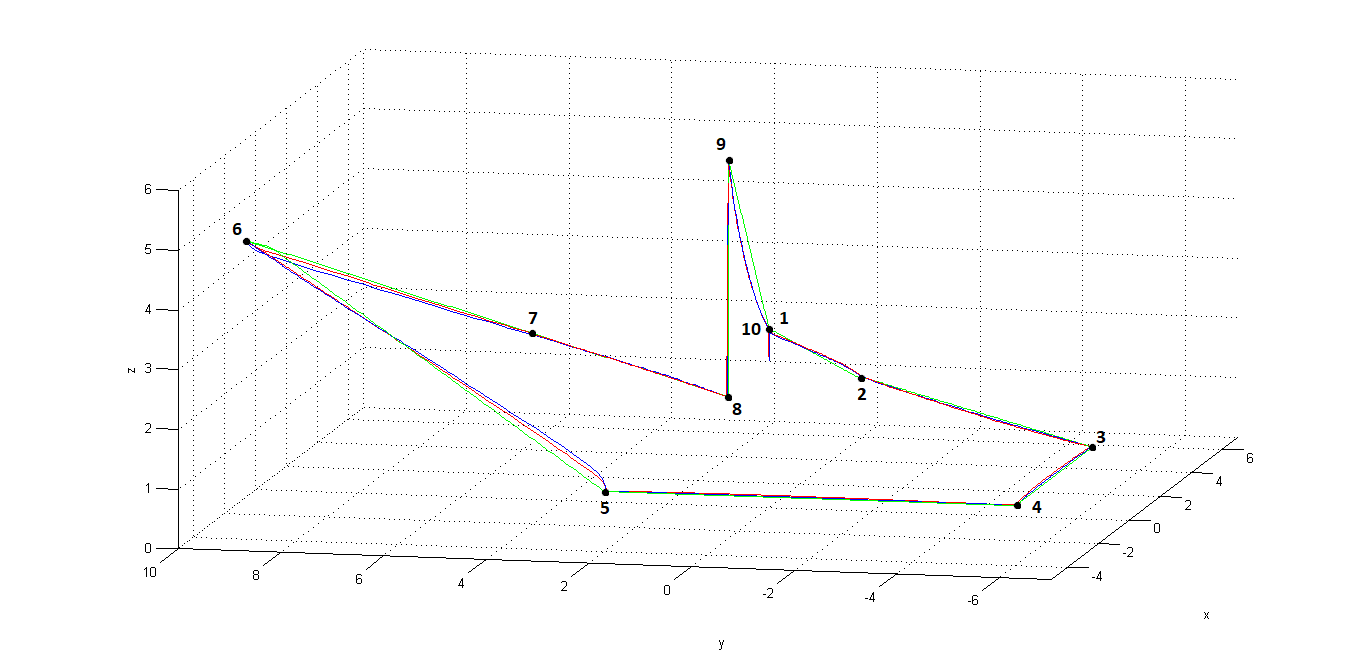
\includegraphics[width=1.1\textwidth]{imag/IMG47.png}
				\caption{Seguimiento de ruta por puntos de paso en 3D.}
		\label{fig:Error asociado al pilotaje.}	
	\end{center}
\end{figure}

\subsection{Pilotaje por trayectorias continuas}
\hspace{1cm} Después de validar el correcto funcionamiento del piloto por puntos se observó que este piloto sólo sería valido para ciertas situaciones concretas de espacios abiertos, por lo que se desarrolló un segundo piloto, el piloto por trayectorias continuas que permite un control más fino de las posiciones del dron. Éste es más complejo ya que tiene variaciones de velocidad lineal y angular (en el ángulo de \textit{yaw}), al introducir giros el sistema presenta comportamientos inestables. Para solucionar este comportamiento se realizó un estudio de relaciones de velocidades y se observó que el rango de velocidades para el funcionamiento estable del sistema de navegación era de [0.3-3.2]m/s. Del mismo modo, los valores de ganancia de giro debían estar comprendidos entre el rango [0.14-0.36]. Esta ganancia de giro era muy importante ya que valores muy altos significaban comportamientos inestables y valores muy bajos no permitían ajustar el giro de forma correcta. 
\\

\hspace{1cm} A continuación se muestran diferentes ejemplos de rutas sencillas y complejas, en los cuales se ha comparado con un piloto anterior, el del PFC de Manuel Zafra \cite{ManuelZafra}, de trayectorias para observar la mejora conseguida tanto reduciendo los errores de distancias a la ruta como acortando el tiempo de realización de rutas.
\\

\hspace{1cm} Empezando con rutas sencillas, en la Figura \ref{fig:Ruta sencilla en trayectoria.} se distinguen: la trayectoria deseada (verde), que es la que se introduce al programa; la trayectoria que realiza el piloto antiguo (azul); y por último, la trayectoria que realiza nuestro piloto (rojo).

\begin{figure}[H]
	\begin{center}
		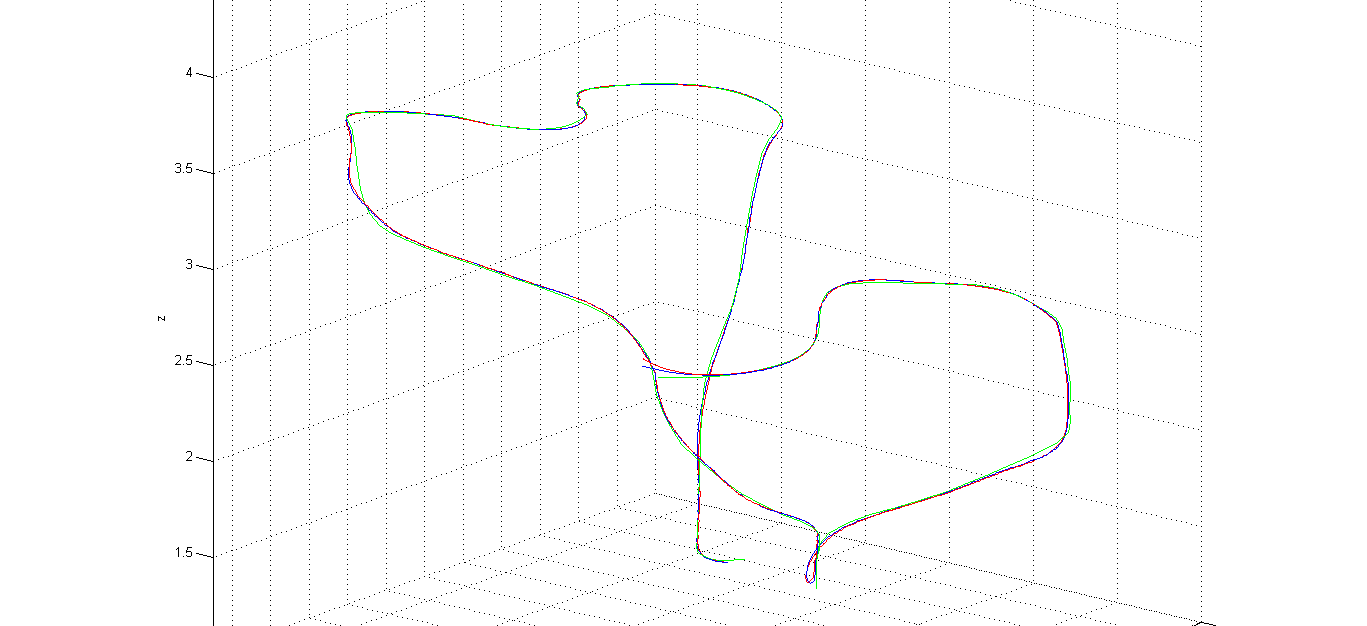
\includegraphics[width=1.1\textwidth]{imag/IMG40.png}
				\caption{Ruta sencilla en el pilotaje por trayectorias.}
		\label{fig:Ruta sencilla en trayectoria.}	
	\end{center}
\end{figure}

\hspace{1cm} En la Figura \ref{fig:Ruta sencilla en trayectoria.} se puede observar cómo ambos pilotos son muy exactos a la hora de realizar las trayectorias deseadas suaves, que no cuentan con cambios de dirección muy bruscos ni con curvas muy cerradas, sobre todo en las partes rectas de las mismas donde se ve como el ajuste es prácticamente perfecto.

\begin{figure}[H]
 \centering
  \subfloat[Piloto Antiguo]{
   \label{f:Piloto Antiguo}
    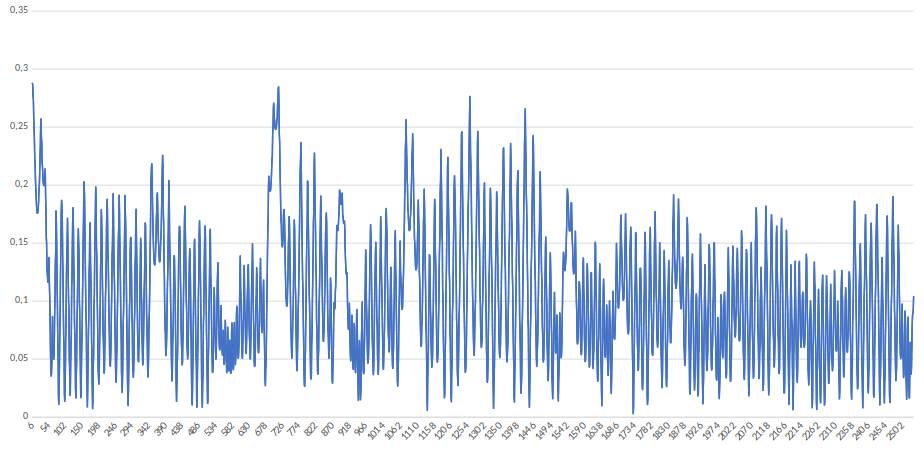
\includegraphics[width=0.5\textwidth]{imag/IMG46.png}}
  \subfloat[Piloto Nuevo]{
   \label{f:Piloto Nuevo}
    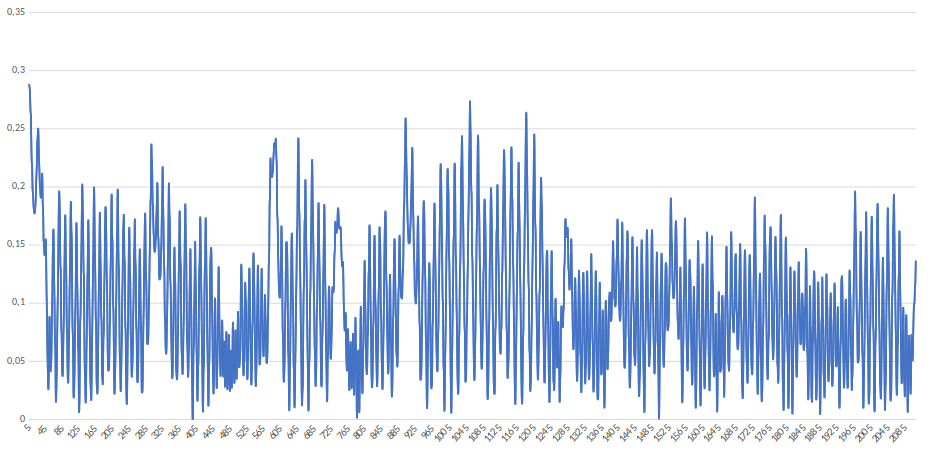
\includegraphics[width=0.5\textwidth]{imag/IMG45.png}} 
 \caption{Comparación del error entre ambos pilotos en ruta sencilla.}
 \label{f:Comparativa del error sencilla.}
\end{figure} 
 
\hspace{1cm} En las gráficas \ref{f:Comparativa del error sencilla.} donde calculando el error obtenemos que el error medio de distancia en nuestro piloto es de 0.1023m con un error máximo en ruta de 0.276m en cambio el piloto antiguo tiene un error medio de 0.1026m y un error máximo de 0.285m. Este error no refleja una diferenciación significativa en cuanto al piloto nuevo y al piloto antiguo en rutas sencillas, en error espacial. Pero sí hay una notable diferencia si nos centramos en el tiempo en que realizan la ruta el piloto nuevo tarda 188.72 segundos mientras que el antiguo utilizaba 253.35 segundos lo que supone una reducción del 25,51\% del tiempo en vuelo, algo muy importante debido a la corta autonomía de los drones.

\begin{figure}[H]
	\begin{center}
		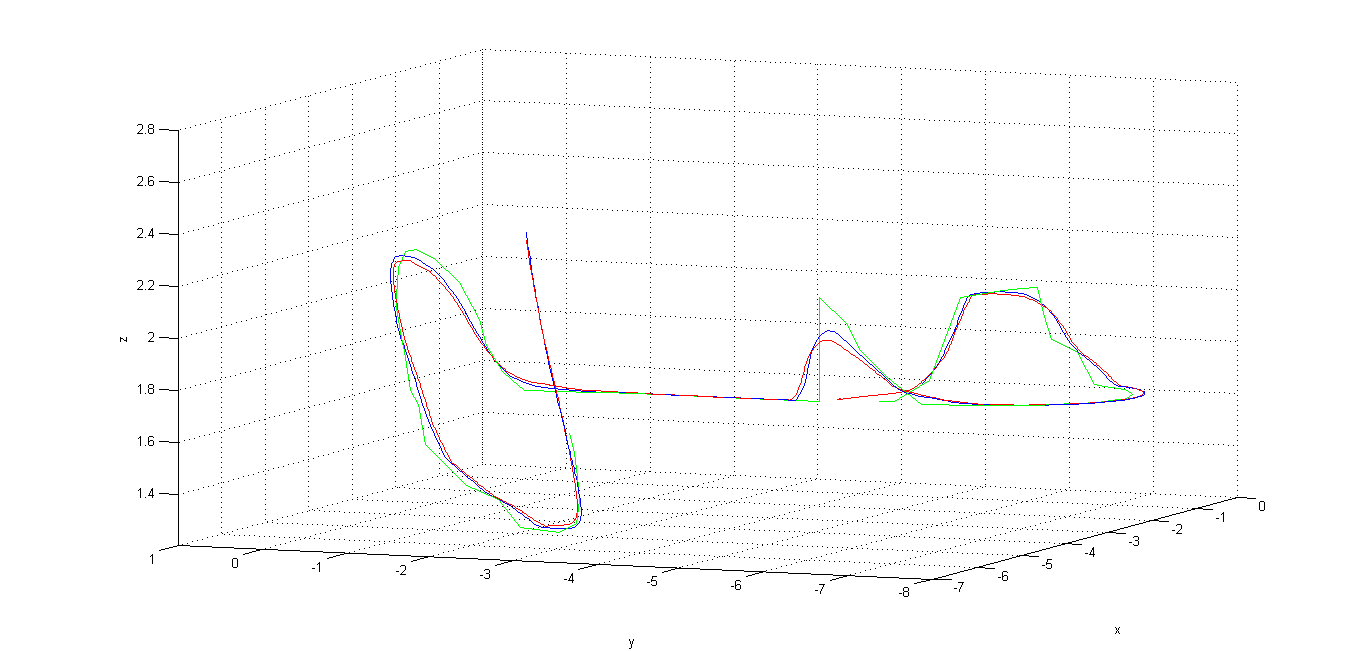
\includegraphics[width=1\textwidth]{imag/IMG41.png}
				\caption{Ruta compleja en el pilotaje por trayectorias.}
		\label{fig:Ruta compleja en trayectoria.}	
	\end{center}
\end{figure}

\hspace{1cm} En cuanto a rutas complejas, para observar mejor el error en distancia, pedimos a los pilotos a una trayectoria con curvas mucho más pronunciadas y con cambios de altitud bruscos. Esta trayectoria se puede observar en la imagen \ref{fig:Ruta compleja en trayectoria.} donde tenemos la trayectoria deseada en verde, el piloto nuevo en azul y el piloto antiguo en rojo. En esta imagen se ve con mayor claridad cómo el piloto nuevo se ajusta mucho más a la ruta deseada. Estas mejores prestaciones se corroboran con los datos de las gráficas de la Figura \ref{f:Comparativa del error compleja.}, en los cuales el error medio del piloto nuevo es de 0.106m y el error máximo es de 0.356m mientras que el error medio del piloto antiguo es de 0.119m con un error máximo de 0.559m. A su vez el nuevo piloto tarda 59.85 segundos en realizar la ruta mientras que el antiguo lo hace en 84.82 segundos reduciendo en este caso el tiempo de ruta en un 29.44\% por lo que en rutas complejas el nuevo piloto se desenvuelve mejor que el antiguo en todos los aspectos.

\begin{figure}[H]
 \centering
  \subfloat[Piloto Antiguo]{
   \label{f:Piloto Antiguo}
    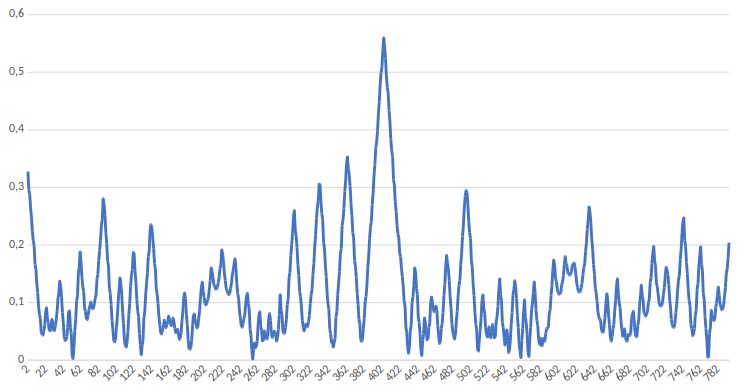
\includegraphics[width=0.5\textwidth]{imag/IMG39.png}}
  \subfloat[Piloto Nuevo]{
   \label{f:Piloto Nuevo}
    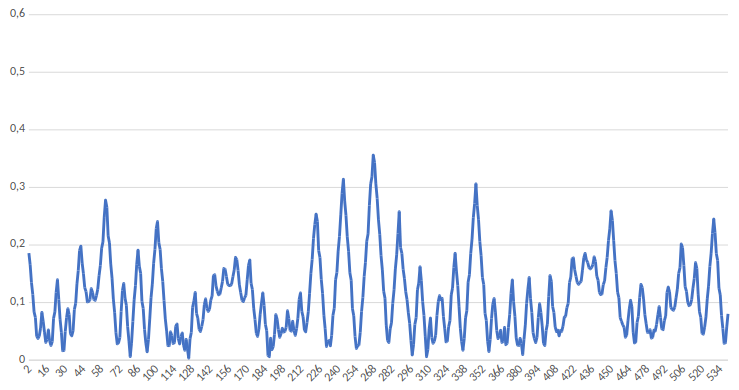
\includegraphics[width=0.5\textwidth]{imag/IMG38.png}} 
 \caption{Comparación del error entre ambos pilotos en ruta compleja.}
 \label{f:Comparativa del error compleja.}
\end{figure} 

\section{Pruebas integrales del sistema}
\hspace{1cm} Una vez conseguido que los componentes por separado funcionasen correctamente, se integraron todos conjuntamente y se realizaron las pruebas finales del sistema. Con ellas se valida experimentalmente la aplicación completa de navegación desarrollada. El buen funcionamiento del sistema se corroboró con los experimentos tanto de la ruta por puntos de paso (en la Figura \ref{fig:Prueba integral de ruta por puntos.}) donde tenemos en verde la ruta deseada, en rojo la posición estimada y en azul la ruta realizada, como de la ruta por trayectorias continuas (en la Figura \ref{fig:Prueba integral de ruta por trayectoria.}). En ambos se ve como el dron seguía la ruta de forma estable y con un margen de error prácticamente nulo, siempre y cuando estén a la vista del vehículo aéreo las balizas AprilTags para su autolocalización. 

\begin{figure}[H]
	\begin{center}
		\includegraphics[width=1.1\textwidth]{imag/IMG42.png}
				\caption{Prueba integral de ruta por puntos.}
		\label{fig:Prueba integral de ruta por puntos.}	
	\end{center}
\end{figure}

\begin{figure}[H]
	\begin{center}
		\includegraphics[width=1.1\textwidth]{imag/IMG43.png}
				\caption{Prueba integral de ruta por trayectoria.}
		\label{fig:Prueba integral de ruta por trayectoria.}	
	\end{center}
\end{figure}

\hspace{1cm} Para el experimento de la navegación integral por trayectoria continua decidimos utilizar una ruta compleja con curvas cerradas y saltos de altura, y así comprobar la integridad y el error de la aplicación para cualquier situación puesto que ése es el escenario de navegación más complejo. En la imagen \ref{fig:Prueba integral de ruta por trayectoria.} se observa la ruta deseada en verde y la ruta realizada en rojo. A primera vista no se aprecian errores demasiado elevados, por lo que analizamos con más detalle lo datos de error de distancia en la Figura \ref{fig:Error de distancia final.}. De este análisis extraemos que el error medio de distancia en esa ruta compleja fue de 0.128m con un error máximo de 0.563m. Este alto error máximo, que es puntual, se debe a que el reconocimiento de las balizas no se puede realizar a velocidades elevadas, el tiempo de ruta fue de 109.5 segundos.

\begin{figure}[H]
	\begin{center}
		\includegraphics[width=0.87\textwidth]{imag/IMG44.png}
				\caption{Error de distancia a la ruta deseada en la prueba integral del sistema}
		\label{fig:Error de distancia final.}	
	\end{center}
\end{figure}

\hspace{1cm} Este error entre la trayectoria ideal y la trayectoria conseguida incluye y acumula dos fuentes de errores independientes: los errores debidos a una mala autolocalización y los errores debidos a un mal pilotaje de los motores del drones. Es interesante destacar que este error medido experimentalmente es similar al que se obtenía cuando se alimenta al pilotaje con las posición 3D perfecta del dron (figura \ref{fig:Prueba integral de ruta por trayectoria.}).
%\lhead[]{CAPÍTULO \thechapter. Conclusiones}
\chapter{Conclusiones}\label{cap.conclusiones}
\hspace{1cm} Una vez expuesto el desarrollo fundamental de este trabajo, en este capítulo vamos a analizar si los objetivos planteados anteriormente se han cumplido. A su vez comentaremos las posibles líneas de desarrollo que partan de este trabajo. Como visión global podemos decir que el trabajo ha sido satisfactorio, ya que se ha conseguido un algoritmo que permita al drone despegar, realizar una ruta y aterrizar, todo ello de manera completamente autónoma, como se deseaba en un primer momento. 

\section{Conclusiones}
\hspace{1cm} En cuanto al análisis de los objetivos vamos a extraer conclusiones sobre cada uno de ellos superado:

\begin{enumerate}
	\item{\textbf{Adaptación e integración del componente Slam-Visualmarkers:} hemos ajustado el componente y lo hemos introducido por pasos para finalmente conseguir su correcto funcionamiento, la nueva aplicación de JdeRobot está implementada en ROS y fruto de este TFG se ha añadido al componente oficial la interfaz del numero de balizas observadas, que permite medir indirectamente la incertidumbre de la estimación de posición.}	
	\item{\textbf{Recodificación e integración del despegue y aterrizaje visual:} El algoritmo permite que el drone despegue de forma controlada estabilizandose sobre la baliza arlequinada, evitando así que se desvíe por factores externos y poder iniciar la ruta deseada con la certeza de que el drone está completamente nivelado. También mencionar que el aterrizaje se ha simplificado para eliminar los temporizadores y la máquina virtual de estados, introduciéndolo correctamente en el nuevo algoritmo.}
	\item{\textbf{Desarrollo de dos módulos de navegación basados en la posición absoluta del drone:} Éxito para ambos controles de pilotaje ya que hemos logrado desarrollar y comprobar que, tanto el método de pilotaje por puntos de paso, en el cual no se controla el giro, como el pilotaje por trayectorias continuas que se
adapta mejor trayectorias complejas y permite un control más fino de la navegación autónoma, funcionan correctamente, con errores mínimos y con una robustez elevada en cualquier tipo de situaciones, demostrando así que se ha creado una mejora con respecto a los anteriores sistemas de pilotaje creados.}
	\item{\textbf{Utilización de la herramienta Visual States:} Se ha logrado desarrollar completamente el algoritmo dentro de esta herramienta, con ello queremos decir que se ha creado la jerarquía necesaria para pasar de un estado a otro mediante transiciones controladas. Por tanto hemos conseguido integrar navegación autónoma, despegue y aterrizaje.}	
	\item{\textbf{Validación experimental en entorno simulado Gazebo:} Todos los resultados obtenidos se han extraído a partir de las pruebas realizadas dentro de los mundos creados en este entorno de simulación tridimensional, tanto con experimentos con pruebas unitarias, como con pruebas integrales. Creando así por tanto ejemplos visuales de la robustez del algoritmo completo, con la utilización de todos los módulos para dotar al sistema de autonomía completa. Mejorando el pilotaje, ligeramente en precisión espacial pero notablemente en la realización de rutas y en el tiempo empleado para ello. Con todo se ha conseguido validar el funcionamiento integral del sistema desarrollado en simulación como un sistema estable y aunque el ruido de las medidas y el comportamiento de los soportes físicos pueden afectar el comportamiento del sistema, este ha probado ser lo suficientemente robusto para satisfacer las metas propuestas dentro de entornos reales.}
\end{enumerate}

\hspace{1cm} Al cumplir el objetivo principal de la aplicación y todos los subobjetivos podemos decir que se ha conseguido mejorar lo existente anteriormente en JdeRobot sobre navegación autónoma de drones. Ahora cuenta con un algoritmo que permite a un drone navegar de forma completamente autónoma desde el despegue hasta el aterrizaje, siguiendo una ruta previamente establecida y utilizando una autolocalización propia, únicamente colocando una serie de balizas y pulsando el botón de inicio.

\hspace{1cm} Antes de extraer las conclusiones sobre los objetivos en el capítulo \ref{cap.objetivos}, mencionar que para conseguirlos se ha hecho uso de un gran número de herramientas y tecnologías que han tenido que ser comprendidas y adaptadas para el propósito buscado. Todas las pruebas y los avances que se han ido desarrollando y validando se pueden ver en la wiki oficial del proyecto \footnote{\url{http://jderobot.org/Jsaizc-tfg}} y el código está accesible en github \footnote{\url{https://github.com/RoboticsURJC-students/2017-tfg-jesus-saiz}} 
\\

\section{Trabajos futuros}
\hspace{1cm} El mundo de la robótica, de la visión artificial y dentro de ambos de los drones, está en constante desarrollo por lo que cada día surgen nuevas necesidades y aplicaciones posibles para este tipo de robots. Este proyecto ha supuesto un aporte, un paso adelante dentro de JdeRobot pero abre a su vez nuevas posibilidades en esta misma línea. A continuación, se detallan algunas de estas líneas de mejora, que han surgido al investigar las herramientas, las nuevas aplicaciones y al desarrollar nuestro propio algoritmo.

\begin{itemize}
	\item Lo primero sería probar el algoritmo en situaciones reales. Aunque hemos comprobado la robustez de algoritmo en entornos simulados y hemos incluido algunas funcionalidades para enfrentarse a entornos reales, no hemos podido comprobar situaciones como: la deriva propia del vehículo, que añade un mayor grado de complejidad al sistema de control; los sistemas de estabilización establecidos por el fabricante, que en ocasiones entran en conflicto con el control proporcionado por el componente; y el ruido de los sensores.
	\item Otra posible linea de investigación es el cambio del sistema de autolocalización visual basado en marcadores por una autolocalización basada en un sistema de odometría visual, evitando así el uso de balizas y localizándonos gracias a la percepción de objetos a nuestro alrededor pudiendo crear incluso mapas en 3D de lo que se encuentra a nuestro alrededor.
	\item Por último, sería interesante extender nuestro algoritmo para adaptarlo a otras necesidades reales como, por ejemplo, capturas de fotografías de puntos estratégicos. Esto puede ser de gran utilidad para su representación posterior en 3D y creación de mapas u objetos e incluso para tareas de vigilancia o monitorización de espacios.
\end{itemize}

\chapter{Bibliografía}

http://www.elai.upm.es/moodle/mod/resource/view.php?id=131

http://blog.sandglasspatrol.com/index.php/articulos/41-militar/758-uavs-clasificacion-tendencias-y-normativa-de-espacio-aereo


\end{document}
